\documentclass[10pt]{report}
\usepackage[table]{xcolor}
\usepackage[utf8]{inputenc}
\usepackage{ngerman}
\usepackage{tikzsymbols}
\usepackage{amsmath}
\usepackage{amsfonts}
\usepackage{amssymb}
\usepackage{graphicx}
\usepackage{geometry}
\usepackage{tikz}
\usepackage{todonotes}
\usepackage{amsthm}
\usepackage{tabularx}
\usepackage{subfiles}
\usepackage{pgfplots}
\usepackage{bbm}
\usepackage{graphicx}
\usepackage{hyperref}
\graphicspath{ {VorlesungenTexDateien/images/} }
\newcommand\tab[1][1cm]{\hspace*{#1}}
    \newcolumntype{L}{>{\raggedright\arraybackslash}X}

		\geometry{a4paper, top=25mm, left=40mm, right=25mm, bottom=30mm,
				headsep=10mm, footskip=12mm}
				\title{Statistisches Lernen\\ \large{Vorlesung Wintersemester 17/18}\\
			}

			\def\firstcircle{(0,0) circle (1.5cm)}
			\def\secondcircle{(45:2cm) circle (1.5cm)}
			\def\thirdcircle{(0:2cm) circle (1.5cm)}
			\date{}
			\author{}
			
				\theoremstyle{definition}
				\newtheorem{exmp}{Beispiel}
				\newtheorem{axiom}{Axiom}
\begin{document}
\maketitle
\tableofcontents

\chapter{Einführung}
	\section{Vorbemerkungen}
	\begin{itemize}
		\item Bei statistischem Lernen geht es darum intelligente Schlüsse aus Daten zu ziehen
		\begin{itemize}
			\item Fokus auf Methoden zu Analysen
			\item wenig/nicht über Design
			\item viele Bsp. aus dem Bereich der klinischen Studien
			\item Anwendungen auf ganz anderen Gebieten
		\end{itemize}
	\item Beispielhafte Anwendungen
	\begin{itemize}
		\item Unterscheiden sich Behandlungen A und B
		\item Was sind die Eigenschaften eines diagnostischen Test
		\item Gibt es einen Zusammenhang zwischen Krankheiten A und B
	\end{itemize}
	\end{itemize}
\section{Wahrscheinlichkeit}
\subsection{Zugänge}
\begin{itemize}
	\item relative Häufigkeit (frequentistisch)
	\item Maß für eine Überzeugung (Bayes'sche Statistik)
\end{itemize}
\textbf{frequentistisch:} intuitiv, basiert auf wiederholbaren ''Experimenten'' (z.B. Münzwurf, radioaktiver Zerfall, Schwangerschaft bei Kontrazeptionsmethode(Verhütungsmethode) A, 5-Jahre Überleben nach Chemotherapie, Regen am nächsten Tag in Leipzig)

\begin{itemize}
	\item in den ersten Vorlesungen folgen wir einem theoretischen Zugang
	\begin{itemize}
		\item dadurch bekommt man ein solides Fundament
		\item wir werden nicht mathematisch streng sein können, (Stichwort Kolmogorow Axiomatik)
	\end{itemize}
\end{itemize}
\subsection{Das Ereignisfeld}
\begin{itemize}
	\item als \textit{Ereignis} bezeichnet man einen möglichen Ausgang eines ''Zufallsexperimentes'', z.B. ''Zahl liegt oben''
	\item Ein System heißt \textit{Ereignisfeld}, wenn:
	\begin{itemize}
		\item es das sichere und das unmögliche Ereignis enthält

				\item A und B Teil eines Systems sind, dann auch $AB$ ($A\cap B$) ''Produkt'' von A und B, bedeutet $x \in A \text{ und } B$
			\item $A+B$ ($A \cup B$) ''Summe'', mindestens eines der Ereignisse A und B tritt ein
			\item $A-B$ ($A\backslash B$) "Differenz'' A tritt ein, während B nicht eintritt

	
	\end{itemize}
\end{itemize}
\begin{exmp}
	Münzwurf Ereignisfeld \{A,B,$\Omega$, $\emptyset$\}\\
	A - Zahl oben\\B - Wappen oben \\ $\Omega$ - Zahl oder Wappen oben \\ $\emptyset$ - weder Zahl noch Wappen oben
\end{exmp}

\subsection{Gesetze der Ereignisse}
\begin{itemize}
	\item Kommutativ: $A+B = B+A$, $AB = BA$
	\item Assoziativ: $A+(B+C)$ = $(A+B)+C$; $A(BC) = (AB)C$
	\item Distributiv: $A(B+C)$ = $(AB)+(AC)$; $A+(BC) = (A+B)(A+C)$ *
	\item Identitäten: $A+A = A$; $AA = A$
\end{itemize}
*(A+B)(A+C) = AA+AC+BA+BC = A+(BC)

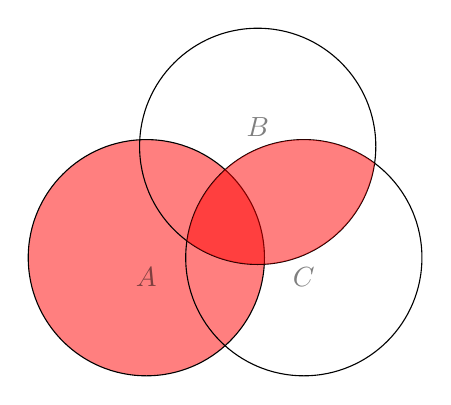
\begin{tikzpicture}
\begin{scope}[shift={(3cm,-5cm)}, fill opacity=0.5]
\fill[red] \firstcircle;

\draw \firstcircle node[below] {$A$};
\draw \secondcircle node [above] {$B$};
\draw \thirdcircle node [below] {$C$};

\clip \secondcircle;
\clip \thirdcircle;
\fill[red]\thirdcircle;
\end{scope}
\end{tikzpicture}

\subsection{Wahrscheinlichkeitsbegriff}
\begin{axiom}
	Jedem Ereignis $A$ aus dem Ereignisfeld $F$ ordnet man eine nichtnegative Zahl $P(A)$ zu. Das ist die \textit{Wahrscheinlichkeit}.
\end{axiom}
\begin{axiom}
	 $P(\Omega)=1$
\end{axiom}
\begin{axiom}
	Sind Ereignisse $A_i$ mit $i\in {1,..,n}$ paarweise unvereinbar (d.h: $A_i A_j = \emptyset$ mit $i \neq j $), so gilt $P(A_1+A_2+ \ldots + A_n) = P(A_1) + P(A_2) + \ldots + P(A_n)$\\

	Daraus ergeben sich folgende Eigenschaften für Wahrscheinlichkeiten:
	\begin{itemize}
		\item $P(\emptyset)= 0$
		\item $P(\bar{A}) = 1 - P(A)$, $\bar{A} = \Omega -A$
		\item $ 0 \leq P(A) \leq 1$
		\item Für $A \subset B$ (A ist Teilereignis von B) folgt $P(A) \leq P(B)$
		\item $P(A+B) = P(A)+P(B)-P(AB)$
		\item  $P(A_1 + A_2+ \ldots +A_n) \leq P(A_1) + P(A_2)+ \ldots+P(A_n)$
	\end{itemize} 	
\end{axiom}

%Vorlesung 2
\subsection{Bedingte Wahrscheinlichkeit}
Eine Wahrscheinlichkeit von A unter der Bedingung dass B eingetreten ist schreibt man als $P(A|B)$
\[P(A|B) = \frac{P(AB)}{P(B)}\]
Motivation: Gegeben seien $n$ unvereinbare, gleich wahrscheinliche Ereignisse \\
\begin{tabular}{ll}
  $A_1,A_2,...,A_n$ & mit $m$ günstig für A \\
 & mit $k$ günstig für B \\ 
 & mit $r$ günstig für AB (r $\leq$ k, r $\leq$ m) \\ 
\end{tabular}
\[ P(A|B)=\frac{r}{k}=\frac{\frac{r}{n}}{\frac{k}{n}}=\frac{P(AB)}{P(B)} \]

\begin{exmp}
	Zwei Würfel werden geworfen. Wie groß ist die Wahrscheinlichkeit die Summe 8 zu erhalten (A), falls bekannt ist, dass die Summe gerade ist(B)\\
	\[ P(A)=\frac{5}{36}, P(B)=\frac{1}{2}, P(AB)=\frac{5}{36} \]
	\[ P(A|B)=\frac{P(AB)}{P(B)}=\frac{5}{18} \]
\end{exmp}


\subsubsection{Bayes'sche Formel} 
Seien $A_1,A_2,...,A_n$ unvereinbar 
\[ P(A_i|B)=\frac{P(B|A_i) P(A_i)}{\sum\limits_{j=1}^n P(B|A_j) P(A_j)} \]

\section{Diagnostische Verfahren - Anwendung von Wahrscheinlichkeit}
Es seien $D^+, D^-$ zwei mögliche Krankheitszustände (krank, gesund) und $T^+,T^-$ die zwei möglichen Ergebnisse eines diagnostischen Tests.
So bezeichnet man:
\begin{itemize}
 \item $P(D^+)$ : Prävalenz
 \item $P(T^+|D^+)$ : Sensitivität
 \item $P(T^-|D^-)$ : Spezifizität
 \item $P(D^+|T^+)$ : positiv-prädiktiver Wert (PPV)
 \item $P(D^-|T^-)$ : negativ-prädiktiver Wert (NPV)
\end{itemize}

\section{Zufallsvariablen und Verteilungsfunktionen}
Qualitative Beschreibung aus Gedenko: ``Eine \underline{Zufallsgröße}(-variable) ist eine Größe, deren Werte vom Zufall abhängen und für die eine Wahrscheinlichkeitsfunktion existiert''\\
Jedem Elementarereignis $\omega \in \Omega$ (unzerteilbar) wird eine reelle Zahl zugeordnet $X=X(\omega) : \Omega = \mathbb{R}$ und $F_x(t):=O(X<t)$ wird als Verteilungsfunktion der Zufallsgröße $X$ definiert. Sie ist monoton nicht fallend, linksseitig stetig und gehorcht den Bedingungen $F(-\infty)=0,F(\infty)=1$ \\
$\rightarrow$ Umkehrung: jede solcher Funktionen lässt sich als Verteilungsfunktion deuten

\section{Wichtige Verteilungsfunktionen}
\textbf{Binomialverteilung}
\[ P_n(m)=\binom{n}{m}p^m q^{n-m} \] 
wobei \[ \binom{n}{m}:=\frac{n!}{m!(n-m)!}, q:= 1-p \] 

\[ F(x)=
  \begin{cases}
    0 & x \leq 0 \\
    \sum\limits_{k<x}P_k & 0 < x \leq n \\
    1 & x > n
  \end{cases}
\] 

\textbf{Poissonverteilung}
\[ P_n=\frac{\lambda e^{\lambda}}{n!}, \lambda > 0 \]

\[ F_{\lambda}(t)=\sum_{k=0}^t \frac{\lambda^k}{k!}e^{-\lambda} \]

\textbf{Normalverteilung}
\[ F(x)=\phi(x)=\frac{1}{\sigma\sqrt{2\pi}} \]

\[ \int_{-\infty}^x e^{\frac{-(z-a)^2}{2\sigma^2}} dz , \sigma > 0 \]

\section{Erwartungswert, Varianz, weitere Momente}
\subsection{Erwartungswert} Sei $E(X)$ eine Zufallsgröße:
\subsubsection{diskret}
$E(X)=\sum_i x_i p_i$ wobei $x_i$: mögl. Werte, $p_i$: Wahrscheinlichkeiten \\

\begin{exmp}
	Würfel 
	\[ E(X)=\frac{1}{6} \sum_{i=1}^6 i = \frac{21}{6} = \frac{7}{2} \]
\end{exmp}
\begin{exmp}
	Binomialverteilung: 
	\[ E(X)= \sum_{k=0}^n k P_n(k) = \sum_{k=0}^n k \binom{n}{k} p^k(1-p)^{n-k} \] 
	Nebenrechnung:
	\[ k \binom{n}{k} = \frac{k n!}{k! (n-k)!} = \frac{n!}{(k-1)!(n-k)!} = \frac{n(n-1)!}{(k-1)!(n-k)!} = n \binom{n-1}{k-1} \] 
	\[\rightarrow E(X)= n \sum_{k=1}^{n} \binom{n-1}{k-1} p^k (1-p)^{n-k} = np \sum_{k=1}^n \binom{n-1}{k-1} p^{k-1} (1-p)^{n-k} \] 
	Sei $k'=k-1, n'=n-1$ \\
	\[ \rightarrow E(X)=np \underbrace{\sum_{k=0}^{n'} \binom{n'}{k'} p^{k'}(1-p)^{n'-k'}}_{=1} = np \]
	
\subsubsection{stetig} 
	\[ E(X)=\int x - p(x) dx , \quad p(x): \text{Wahrscheinlichkeitsdichte} \]
\end{exmp} 

\begin{exmp}
	Uniformverteilung auf Intervall $[a,b]$
	\[ E(X)= \frac{1}{b-a} \int_{a}^b x dx =  \frac{b^2 - a^2}{2(b-a)} = \frac{1}{2}(b+a) \]
\end{exmp}


\begin{exmp}
	Normalverteilung
\[ E(X)= \frac{1}{\sigma \sqrt{2 \pi}} \int_{-\infty}^{\infty} x e^{\frac{-(x-a)^2}{2\sigma^2}} dx \]
\[ x' = \frac{x-a}{\sigma} \rightarrow x = \sigma x' + a ,\quad dx= \sigma x' \]
\[ E(X) = \frac{\sigma}{\sigma \sqrt{2 \pi}} \int_{- \infty}^{\infty} (\sigma x' + a) e^{\frac{-x^2}{2}} dx' \]
ungerade Funktion ergibt 0
\[ E(X) = \frac{\sigma}{\sqrt{2 \pi}} \underbrace{\int_{- \infty}^{\infty} e^{-x' 2/2} dx'}_{=\sqrt{2 \pi}} = a \]
\end{exmp}

\subsection{Varianz} (oder Dispersion)
\[ V(X) := E \big[ (X-E(X)^2) \big] \]
\underline{diskret}: 
\[ V(X) = \sum\limits_{i} \big[ x_i - E(x) \big] ^2 * p_i \]
\underline{stetig}: 
\[ V(X) = \int \big[ x_i - E(x) \big] ^2 * p(x)\; dx \]


%Vorlesung 3
\[
V(X) := E[(EX)-X)^2] = E[E(X)^2 - 2X E(X) + X^2]  = E(X^2) - [E(X)]^2
\]
Bsp. Würfel
\[
V(X) = \dfrac{1}{3} \left[\left(\dfrac{5}{2}\right)^2 + \left(\dfrac{3}{2}\right)^2 + \left(\dfrac{1}{2}\right)^2\right] = \dfrac{35}{12}
\]
Bsp. Uniformverteilung [a,b]
\begin{align*}
V(X) &= \dfrac{1}{b-a} \int_a^b \! x^2 \, \mathrm{d}x - \left(\dfrac{b+a}{2}\right)^2\\
&= \dfrac{b^3 - a^3}{3 (b-a)} - \dfrac{(b+a)^2}{4} \\
&= \dfrac{(b-a) (b^2+a^2+ab}{3(b-a)} - \dfrac{(b+a)^2}{4}\\
&= \dfrac{1}{12} (4b^2+4a^2+4ab-3b^2-6 ab-3a^2)\\
&= \dfrac{1}{12} (b^2-a^2-2ab) \\
&= \dfrac{(b-a)^2}{12}
\end{align*}
\paragraph{Definition:}
Wir bezeichnen $m_k$ als das \underline{gewöhnliche Moment} (oder Anfangsmoment)\\
k-ter Ordnung \[m_k := E(X^k),\] \\
diskret \[\sum_i\left(x_i\right)^k p_i,\]
stetig \[\int \! x^k p(x) \, \mathrm{d}x\]

\paragraph{Definition:}
Das \underline{zentrale Moment} (auf Zentrum Erwartungswert bezogen) k-ter Ordnung \[\mu_k := E\left[(X-m_1)^k\right]\]. \\
Die Varianz ist also das zweite Zentralmoment \[V(X) = \mu_2 = m_2 - (m_1)^2\].\\
Man kann immer $\mu_k$ durch $m_l$ $\left( l \leq k\right)$ ausdrücken.

\subsection{Korrelation}
Eine Erweiterung dieser Momente stellt die \underline{Kovarianz} dar (gemischte Zentralmomente zweiter Ordnung).
\[
b(X,Y) := E\left[\left(X-E(X)\right) \left( Y-E(Y) \right)\right]
\]

Es gilt offensichtlich $b(X,X) = V(X)$.\\
Die normierte Größe $\rho(X,Y)$ mit 
\[\rho(X,Y) := \rho_{X,Y} = \dfrac{b(X,Y)}{\sqrt{V(X)V(Y)}}\]
bezeichnet man als \underline{Korrelationskoeffizient}. \\
Es gilt: $-1 \leq \rho \leq 1$.\\ Für $X=Y$ gilt $\rho = 1$ und für $X=-Y$ gilt $\rho = -1$. \\
Falls $X$ und $Y$ unabhängig dann gilt $\rho = 0$ (nicht aber umgekehrt).
\subsubsection*{Anwendung auf Wahrscheinlichkeiten:} 
\begin{align*}
E(X) &= p_X\\
V(X) &= p_X(1 - p_X)\\
\rho_{X,Y} &= \dfrac{p_{XY} - p_Xp_Y}{\sqrt{p_X(1-p_X) p_Y(1-p_Y)}}\\
\rightarrow p_{XY} &= p_Xp_Y + \rho_{X,Y} \sqrt{p_X(1-p_X)p_Y(1-pY)}
\end{align*}
\textbf{Grenzfälle} 
\begin{align*}
\rho &= 0 : p_{XY} = p_X p_Y\\
\rho &= 1 \footnote{$\rightarrow p_X = p_Y$} : p_{XY} = (p_X)^2 + p_X(1-p_X) = p_X\\
\rho &= -1 \footnote{$\rightarrow p_X = 1 - p_Y$} : p_{XY} = p_X(1-pX) - p_X(1-p_X) = 0 \\
\end{align*}

\section{Einige wichtige Gesetze der Wahrscheinlichkeitstheorie}
\subsection{Gesetz der großen Zahlen}
\textbf{Bernoulli:} Für alle $\epsilon > 0$ :
\[ \lim\limits_{n \rightarrow \infty}{P \left\lbrace| \dfrac{\mu}{n} - p | < \epsilon \right\rbrace} = 1\]
\begin{itemize}
	\item $\mu$ - Anzahl der Ereignisse
	\item $n$ - Anzahl der Versuche
	\item $p$ - Wahrscheinlichkeiten der Ereignisse
\end{itemize}
%Vorlesung 4
\textbf{Tschebyshew:} Für ein $\epsilon > 0$:
\[\lim\limits_{n \to \infty} P \left\{\frac{1}{n} \sum_{i=1}^{n} X_i - \frac{1}{n} \sum_{i=1}^{n} E(X_i)| < \epsilon \right\} = 1\] 
für eine Folge paarweise unabhängiger Zufallsgrößen.\\

$\{X_i\}_{i=1,2, \ldots n}$ mit gleichmäßiger beschränkter Varianz  $V(X_i) \leq C$


\subsection{lokaler Grenzwertsatz von Moivre-Laplace}
Sei $0<p<1$ die Wahrscheinlichkeit eines Ereignisses.
In n-Versuchen gilt
\[P_n (m) = \binom{n}{m} p^m(1-p)^{n-m}\] So gilt \[\lim\limits_{n \to \infty} \frac{\sqrt{np(1-p)} P_n(m)}{\frac{1}{\sqrt{2 \pi}} e ^{-\frac{x^2}{2}}} \rightarrow  1 \text{ mit } x=\frac{m-np}{\sqrt{np(1-p)}}\]

\subsection{zentraler Grenzwertsatz}

Sei \[S_n =  \sum_{i=1}^{n} X_i\]
mit $E(X_i)<\infty$, $V(X_i) = \sigma ^2 < \infty$. So gilt für jedes t
\[ \lim\limits_{n \rightarrow \infty} P \left(\frac{S_n - n \cdot E(X_i)}{\sigma \sqrt{n} }< t\right) = \frac{1}{\sqrt{2\pi} }\int_{-\infty}^{t} e^{\frac{-x^2}{2}} dx
\]

also: die Folge der Verteilungen der standardisierten Zufallsgröße konvergiert gegen die Standartnormalverteilung (d.h. a = 0, $\sigma$ = 1)

\chapter{Deskriptive Statistik}
\begin{itemize}
	\item Beschreibung von Daten und Kohorten ist zentral für das Verständnis einer Arbeit
	\item Ziel ist mit wenigen Kenngrößen das wesentliche zu charakterisieren 
	\item man gibt ''Punktschätzer''  für Erwartungswerte und ''Konfidenzintervalle'' (KI; engl. CI) als Maß für die Genauigkeit der Schätzung:
	\[(1- \alpha) \text{ KI} [a,b] : P(a \leq \theta \leq b) = 1-\alpha\]
\end{itemize}
\section{Nominale und Ordinale Größen}
%nominal -- Kann man nur kategorisieren aber nicht ordnen
%ordinal -- ist eine Kategoriale Größe die man in eine Reihenfolge bringen kann

\begin{itemize}
	\item absolute und relative Häufigkeiten (z.B Häufigkeitstabellen)
	\item grafisch: Balkendiagramme (mit Konfidenzintervall KI oder Standardfehler SE)
	\item Kreisdiagramm (verpönt)
\end{itemize}
\begin{align*}	
	\hat{p} &= \frac{r}{n}\\
	\hat{SE} &= \frac{\hat{sd}}{\sqrt{n}}= \frac{\sqrt{\hat{V}}}{\sqrt{n}} = \sqrt{\frac{\hat{p} (1- \hat{p})}{n}}
	KI \approx \hat{p} \pm 2 SE,
\end{align*}
r= \#Fehlgeburten, n = \#Beobachtungen 



\section{Metrische Daten}
\textbf{Lagemaß}
\begin{itemize}
	\item Mittelwert (arithmetisch oder geometrisch, d.h. log-Skala)
	\begin{itemize}
		\item übliche und ''robuste'' Methoden
		\item arithmetisch  = $\frac{1}{n}\sum_{i=1}^{n} X_i$
		\item geometrisch  = $[ \prod_{i=1}^{n} X_i]^{1/n}$
	\end{itemize}
	-Median und andere Quantile (verschiedene Schätzverfahren)
\end{itemize}
\textbf{Streumaß}
\begin{itemize}
	\item Standardabweichung (''sample'' - Methode) $sd^2 = \frac{1}{n-1} \sum_{i=1}^{n}(x_i - \bar{x})^2$
	\item Interquartilabstand (engl. interquartile range (IQR) z.B. 25. und 75. Perzentil)
	\item Spannweite
	\item grafisch: Histogramm, Boxplot	
\end{itemize}

\section{Zusammenhang 2er Merkmale}
Nominal
\begin{itemize}
	\item Kontigenztafel: odds ratio, relatives Risiko
	\item grafisch: forest plots
\end{itemize}
metrisch
\begin{itemize}
	\item Korrelationskoeffizient (mit KI)
	\item Streudiagramm
\end{itemize}

\paragraph{Simpsons Paradoxon}
Grundidee: Effekt in Gesamtgruppe muss nicht ''echt'' sein. Er kann in Subgruppen anders ausfallen.

\begin{tabular}{|c|c|c|}
	\hline 
	& A & B \\ 
	\hline 
	Erfolg & 70 (30\%) &  50(22\%) \\ 
	\hline 
	Misserfolg & 160 & 182 \\ 
	\hline 
	Summe & 230 & 232 \\ 
	\hline 
\end{tabular} 

\begin{tabular}{|c|c|c|c|}
	\hline 
	&   & A & B \\ 
	\hline 
	Männer & E & 7 (20\%) & 45(21\%) \\ 
	\hline 
	& M & 28 & 175 \\ 
	\hline 
	Frauen & E & 63(32\%) & 5(33\%) \\ 
	\hline 
	& M  & 132 & 10 \\ 
	\hline 
\end{tabular} 


\chapter{Statistisches Testen}
\section{Die Logik des Testes}
Die Analogie zum Beweis durch Widerspruch kann hilfreich sein, hier ein Beispiel:\\
\begin{tabularx}{\linewidth}{|L|L|}  
	\hline
	Statistisches Testen & Beweis durch Widerspruch \\ \hline
	-Annahme: $H_0: \mu_1 = \mu_2$ (Mittelwert d. Gruppe 1 ist MW d. Gruppe 2)  & -Annahme: $\sqrt{2}$ ist rational \\
	-man glaubt nicht an Annahme & -man glaubt nicht an Annahme \\
	-Folge: Wenn Ann. stimmt... & -Folge: Wenn Ann. stimmt... \\
	-Kommt etwas sehr Unwahrscheinliches raus, so ist die Annahme nicht plausibel(Konvention $< 5\%$ dann wird $H_0$ abgelehnt) & -Kommt man auf einen Widerspruch, so muß die Annahme falsch sein \\
	-Kommt etwas Plausibles raus, so weiß man wenig über die Annahme (KI kann helfen) & -Kommt man nicht auf einen Widerspruch, so weiß man evtl. wenig über die Annahme \\ \hline
\end{tabularx}
\begin{tabularx}{\linewidth}{|L|L|L|}
	\hline
	& $H_0$ stimmt & $H_0$ stimmt nicht \\ \hline
	$H_0$ abgelehnt & Typ I Fehler \newline $\alpha$ \newline (Konvention $\alpha = 0.05$) & \dSmiley \newline Power: $1-\beta$ \\ \hline
	$H_0$ nicht abgelehnt & \dSmiley & Typ II Fehler\newline $\beta$ \newline Planung: $\beta=0.1 ... 0.2$ erstrebt... \newline Sicherheit über $\beta$ hat man nicht \\ \hline
\end{tabularx}

\section{Der T-Test}
Vergleich zweier MW, $H_0: \mu_1 = \mu_2$ \\
Wir schätzen die ``t-Statistik'' (Annahme gleicher Varianz) \\
\[ T = \frac{\bar{x}_1 - \bar{x}_2}{s \sqrt{\frac{1}{n_1} + \frac{1}{n_2}}} \]
\[ s^2 = \frac{(n_1 - 1) s_1^2 + (n_2 -1) s_2^2}{n_1 + n_2 -2} \]
n: Stichpunktgröße der i-ten Gruppe \\
$\bar{x}_i$: MW \\
$s_i^2 = \sum\limits_{j=1}^{n_i} (x_j^{(i)} - \bar{x}^{(i)} )^2 $ \\
($T = \frac{\Delta}{SE}$ ist die grundlegende Struktur) \\
Unter $H_0$: T hat ``t-Verteilung'' mit f-Freiheitsgraden
\[ f= n_1 + n_2 -2 \]
Welch-Test (keine Annahme zur Varianz) \\
\[ T = \frac{\bar{x}_1 - \bar{x}_2 }{\sqrt{\frac{s_1^2}{n_1} + \frac{s_2^2}{n_1}}} \]
t-Verteilung mit f Freiheitsgraden
\[ f=\frac{(\tilde{s_1}^2 + \tilde{s_2}^2)^2)}{\frac{\tilde{s_1}^4}{n_1 - 1} + \frac{\tilde{s_1}^4}{n_1 - 1}} \]
\[ \tilde{s_i} = \frac{s_i}{\sqrt{n_i}} \]
KI für $\Delta \mu$: $\Delta \bar{x} \pm \underbrace{t_{\alpha / 2 , f}}_{\sim 2 \text{ für } \alpha=0.05 \text{ und } f >> 1}  \cdot$ SE \\
p-Wert: Wahrscheinlichkeit den Wert von T zu beobachten unter $H_0$ \\
Ist der p-Wert $p_0$, so beinhaltet ein $(1-p_0)$-KI gerade so den Wert Null \\
z.B. Ist $p_0=0.05 \rightarrow$ das 95\%-KI erreicht die Null gerade so

\section{Kontingenztafel: $\chi^2$- und Fischer-Test}
Gegeben sei:
\begin{tabular}{c|c|c|c}
	& A & B \\ \hline
	I & $n_{11}$ & $n_{12}$ & $n_{1\cdot}$ \\ \hline
	II & $n_{21}$ & $n_{22}$ & $n_{2\cdot}$ \\ \hline
	& $n_{\cdot1}$ & $n_{\cdot2}$ & $n_{\cdot\cdot}$
\end{tabular}
\newline
$\frac{n_{11}}{n_{21}}$ schätzt das ``Odds'' (die Chance) von I im Vergleich zu II bei Gruppe A. \\
$\widehat{OR}=\frac{\frac{n_{11}}{n_{21}}}{\frac{n_{12}}{n_{22}}}$ schätzt das ``Odds Ratio'' (Chancenverhältnis) KI: $OR \cdot e^{\pm z_{a/2} \cdot SE}$ \\
Hier ist die Frage, ob 1 im Intervall liegt (Null auf der log-Skala)\\
Fisher-Test $\Leftrightarrow$ KI von OR (mit anderer Schätzmethode allerdings)  \\
Fischer-Test heißt ``exakt'', da ein strenger Wert aus der Kombinatorik berechnet wird
\[ p = \frac{\binom{n_{1\cdot}}{n_{11}} \binom{n_{2\cdot}}{n_{22}}}{ \binom{n_{\cdot \cdot}}{n_{\cdot1}}} \]
\[ \binom{n_{\cdot\cdot}}{n_{\cdot1}} = \frac{n_{12} + n_{22} + n_{12} + n_{21} }{n_{12} + n_{21} } \]

%Vorlesung 6
Der Zusammenhang nominaler Merkmale kann mit höherer Power mit dem (asymptotischen) $\chi^2$-Test als mit einem exakten Test überprüft werden.
\[ \chi^2 = \sum\limits_{i,j} \frac{(n_{ij} - e_{ij})^2}{e_{ij}} \]
\[ e_{ij}= \frac{n_{i\cdot} \times n_{\cdot j}}{n_{\cdot \cdot}} \]
$e_{ij}:$ erwartete Anzahl \\
$\chi^2$ hat $\chi^2$-Verteilung mit $f=(l-1)\cdot(k-1)$ Freiheitsgrade  \\
(wobei l= Anzahl an Zeilen, k= Anzahl Spalten der Kontigenztafel) \\
Faustregel: $n_{ij} \neq 0$ für alle $i,j$ und $< 20 \%$ der Zellen haben $l_{ij} < 5 \rightarrow \chi^2$-Test \\
%Ende der Vorlesung

\section{Multiples Testen}
%\section{Rückblick}
%\textbf{Hypothese:} \begin{itemize}
%	\item [$\theta$] -Parameter von Interesse (z.B. $\theta = \mu$, $\theta = \sigma^2$, $ \theta = \beta_j $ , ....)
%	\item[$\Theta$] Parameterraum für Parameter $\theta$ (z.B. $ \Theta = \mathbb{R}, \Theta = \mathbb{R}_+, \Theta= [0,1] $ ) 
%\end{itemize}
%Zerlegung vom $ \Theta $ in $ \Theta_0 $ und $ \Theta_A $, sodass gilt
%\begin{itemize}
%	\item $ \Theta_0 \cup \Theta_A = \Theta $
%	\item $ \Theta_0 \cap \Theta_A = \emptyset $
%	\item[$ \rightarrow $] $H_0$ $\theta \in \Theta_0 vs. H_a \theta \in \Theta_A $
%\end{itemize}
%(z.B $ \theta = \mu $,  $ \Theta = \mathbb{R} $, $ \Theta_0 := {0} $ , $ \Theta_A = \mathbb{R} \ {0} $)\\\\
%\textbf{Test:} 
%\begin{itemize}
%	\item[] $ S^n $  -Raum aller n-elementigen Stichproben
%	\item[] $ X = X_1,\ldots X_n)^T \in S^n $  -Stichprobe
%	\item[] $ \phi : S^n \rightarrow {0,1} $ -Test, Abbildung von $ S^n $ - nach 0 bzw. 1
%\item[$ \rightarrow $] Konvention: 
%\begin{itemize}
%	\item[]$ \phi(X) = 1 \Leftrightarrow H_0 $ wird verworfen
%	\item[]$ \phi(X) = 0 \Leftrightarrow H_0 $ wird nicht verworfen
%\end{itemize}
%\end{itemize}
%\textbf{Fehler:} 
%\begin{itemize}
%	\item Fehler 1.Art ($\alpha$ - Fehler, Typ 1 Fehler)
%	\begin{itemize}
%		\item $H_0$ ablehnen, obwohl $H_0$ gilt
%		\item[$\rightarrow $] $\phi(X)=1$ aber $\theta \in \Theta_0$
%	\end{itemize}	
%	\item Fehler 2.Art ($\beta$-Fehler, Typ 2 Fehler)
%	\begin{itemize}
%		\item $H_0$ nicht ablehnen, obwohl $H_0$ nicht gilt
%		\item[$\rightarrow$] $\phi(x) = 0$ aber $\theta \in \Theta_A$
%	\end{itemize}
%\end{itemize}
%\textbf{Vorgehen:}
%\begin{enumerate}
%	\item Festlegen einer oberen Schranke $\alpha$ für den Fehler 1. Art (z.B. $\alpha$ = 5\% = 0.05)
%	\item mit $\alpha$ auch 1. minimierung der Wahrscheinlichkeit $\beta$ für einen Fehler 2. Art
%\end{enumerate}

\paragraph{Multiples Testproblem}

\begin{tikzpicture}
\begin{axis}[%
xlabel={x},
ylabel={y},
xtick={0.2,0.4,0.6,0.8,1.0},
ytick={0.2,0.4,0.6,0.8,1.0},
xmin=0.0, xmax=1.0,
ymin=0.0, ymax=1.0,
xticklabels={$\alpha_1$,$\alpha_2$,$\alpha_3$,$\alpha_4$,$\alpha_5$,$\alpha_6$,$\alpha_7$},
yticklabels={}
]
\addplot [thick,blue] coordinates {
(0.0, 0.0) (0.2,0.0)
(0.2, 0.0) (0.4,0.2)
};
\addplot [dashed,red] coordinates {
(0.0, 0.0) (0.4,0.0)
(0.4, 0.0) (0.6,0.2)
};
\end{axis}
\end{tikzpicture}

\begin{exmp}
	Genetik, SWAS
	\begin{itemize}
		\item 500 000 SNPs werden auf Assoziation mit einem Phänotypen getestet
		\item $\alpha = 5\%$ $\rightarrow$ ca. 25 000 falsch positive Ergebnisse
	\end{itemize}
\end{exmp}
Gegeben:
\begin{itemize}
	\item $X= {X_1, X_n}^T \in S^n$ - Stichprobe,
	\item $\theta$ -interessierende Parameter,
	\item $\Theta$ Parameterraum für $\theta$
\end{itemize}
$\mathcal{H}_0 := \{ H_0^{(j)} \subseteq \Theta$ , $j \in \{1, \ldots, m\} \}$ - Menge von Nullhypothesen\\
$\mathcal{H}_A := \{ H_A^{(j)} = \Theta \ H_0^{(j)} , j \in \{1, \ldots, m\}\}$ - Menge der entsprechenden Alternativhypothesen
\begin{itemize}
	\item[$\rightarrow$] Ein multipler Test ist ein Vektor 
	\item[]$\phi = (\phi_1, \phi_n)^T: S^n \mapsto \{0,1\}^m$ 
wobei jedes $\phi_j$ mit $j \in \{1,m\}$ ein Test ist ($\phi_j: S^n \mapsto \{0,1\}$) auf Grundlage der Stichprobe $X = (X_1,\ldots, X_1)^T$
\end{itemize}
\textbf{Interpretation}
\begin{itemize}
	\item Sei $\theta \in \Theta$ der wahre Parameter.
	\item[$\rightarrow$] $H_0^{j}$  gilt $\Leftrightarrow \theta \in H_0^{(j)} \subseteq \Theta$
	\item[$\rightarrow$] $H_0^{j}$ gilt nicht $\Leftrightarrow \theta \in H_A^{(j)} \subseteq \Theta \ H_0^{(j)} $
mit $j \in \{1,\ldots,m\}$
	\item[]$I_0(\theta) := \{j \in \{1,m\} : \theta \in H_0^{(j)} \}$ - Menge der unter $\theta$ wahren Nullhypothesen
	\item[]$I_A(\theta) := \{j \in \{1,m\} : \theta \in H_A^{(j)} \}$ - Menge der unter $\theta$ wahren Alternativhypothesen
\end{itemize}

%Vorlesung vom 23.11.17

\subsection{Family-wise Error Rate (FWER) }
\[ \text{FWER}_{\theta}(\phi)  := P \left( \bigcup_{j\in I_{0}(\theta)} \{ \phi_j = 1\} \right) \]
$\mathrel{\widehat{=}}$ Wahrscheinlichkeit für einen multiplen Fehler 1.Art (falls $\theta$ der wahre Parameter ist) \\
$\rightarrow \phi$ heißt \underline{Test zum multiplen Niveau $\alpha$ }, falls
\[ \text{FWER}_{\theta}(\phi) \leq \alpha \]
für alle $\theta \in \Theta $

\subsection{Kontrollierende Verfahren für FWER}
\paragraph{Bonferon}
\[ \phi = (\phi_{1},...,\phi{m})^T \text{  - multipler Test} \]
\[ P(\{\phi_j = 1\} \leq \underbrace{\frac{\alpha}{m}}_{\text{Bonferoni-Korrektur}} \text{ für alle } \theta \in H_0^{(j)}, j \in \{1,...,m\} \]
\[ \Rightarrow \text{FWER}_{\theta}(\phi) \leq \alpha \text{ für alle }\theta \in \Theta \]
$\rightarrow$ Ist jedes $\phi_j, j \in \{1,...,m\}$ ein Test zum Niveau $\tilde{\alpha} := \frac{\alpha}{m}$, so ist $\phi$ ein multipler Test zum Niveau $\alpha$

\paragraph{\v Sid\'ak}
\begin{itemize}
 \item $ \phi = (\phi_{1},...,\phi{m})^T \text{  - multipler Test} $
 \item $\phi_j (X), j \in \{1,...,m \}$ unabhängig
\end{itemize}
\[ P(\{\phi_j = 1\} ) \leq 1-(1-\alpha)^{\frac{1}{m}} \text{ für alle } \theta in \Theta, j \in \{1,...,m\}\]
\[ \Rightarrow \text{FWER}_{\theta}(\phi) \leq \alpha \text{ für alle }\theta \in \Theta \]
$\rightarrow$ Ist jedes $\phi_j, j \in \{1,...,m\}$ ein Test zum Niveau $\tilde{\alpha} := 1-(1-\alpha)^{\frac{1}{m}}$ und sind alle Tests voneinander unabhängig so ist $\phi$ ein multipler Test zum multiplen Niveau $\alpha$ \\
Es gilt:
\[ \frac{a}{m} \leq 1-(1-\alpha)^{\frac{1}{m}} \]
$\rightarrow$\v Sid\'ak ist weniger konservativ als Bonferoni, wenn die Tests unabhängig voneinander sind \\

\paragraph{p-Wert:}
Der p-Wert ist die Wahrscheinlichkeit dafür, dass unter der Nullhypothese die Prüfgröße T (statistischer Test) den Wert T(x) oder einen extremeren Wert annimmt, wobei $x-(x_1,...,x_n)^T$ die Realisierung der Stichprobe $X=(X_1,...,X_n)^T$ ist
\begin{center}
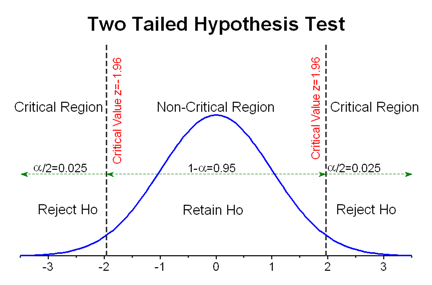
\includegraphics[scale=0.8]{twotailedtest.png}
\end{center}

\paragraph{Bonferroni-Holm-Test}
\begin{itemize}
 \item $\phi=(\phi_1,...,\phi_m)^T $ - multipler Test
 \item $\phi=(p_1,...,p_m)^T $ - zu Tests gehörende p-Werte
 \item $p_{(1)} \leq ... \leq p_{(m)} $ - geordnete p-Werte
 \item $H_{(1)},...,H_{(m)} $ - zu geordneten p-Werten gehörende Nullhypothesen
 \item $\tilde{\alpha}_j := 
	\begin{cases}
	 \frac{a}{j} & , \text{ falls } p_j(X) \text{ nicht unabhängig } \\
	 1-(1-\alpha)^{\frac{1}{j}} & , \text{ falls } p_j(X) \text{ unabhängig }
	\end{cases}
	$
 \item $\phi^{BH}=(\phi_1^{BH},...,\phi_m^{BH})^T$ mit \\
 $\phi_j^{BH} := 
      \begin{cases}
       1 & ,\text{ falls } j \leq j^* \\
       0 & ,\text{ falls } j > j^* \\
      \end{cases}
      $\\
      wobei $j^* =\max\{ \max\{j \in I_0(\theta) \cdot p_{(k)} \leq \tilde{\alpha}_{m-k+1}$ für alle $k \in \{1,...,j\}\}, 0 \}$
\end{itemize}
\paragraph{Beispiel}
\[ p_{(1)} \leq \frac{\alpha}{m} = \tilde{\alpha}_1 \]
\[ p_{(2)} \leq \frac{\alpha}{m-1} = \tilde{\alpha}_1 \]
\[ p_{(3)} \textcolor{red}{>} \frac{\alpha}{m-2} = \tilde{\alpha}_1 \]
\[ p_{(4)} > \frac{\alpha}{m-3} = \tilde{\alpha}_1 \]
\[ p_{(5)} \leq \frac{\alpha}{m-4} = \tilde{\alpha}_1 \]
$\Rightarrow \phi^{BH}$ ist multipler Test zum multiplen Niveau $\alpha$  \\
\textbf{Info:} \\
Bonferroni-Holm ist beser als Bonferroni bzw. \v Sid\'ak bzgl. Typ-II-Fehlern\\
$\rightarrow$ ''step-down''-Verfahren

\section{False Discover Rate (FDR) }
\begin{minipage} [t] {0.6\textwidth}
\begin{tabular}{c|c|c|c}
0-Hyp\ Test & nicht ablehnen & ablehnen & \\ \hline
wahr & \cellcolor{yellow!25} $m_0 (\theta) - V(\theta)$ & \cellcolor{yellow!25}$V(\theta)$ & \cellcolor{yellow!25}$m_0(\theta)$\\ \hline
falsch &\cellcolor{yellow!25}$m_A (\theta) - S(\theta)$  &\cellcolor{yellow!25} $S(\theta)$ &\cellcolor{yellow!25} $m_A(\theta)$\\ \hline
& \cellcolor{red!25}$m-R(\theta)$ & \cellcolor{red!25}$R(\theta)$ & m\\
\end{tabular}
\end{minipage}
\begin{minipage} [t] {0.3\textwidth}
gelb=unbekannt\\ rot=bekannt
\end{minipage}

\begin{itemize}
 \item $m$ - Anzahl der Tests \\
 \item $m_0 (\theta)$ - Anzahl der unter $\theta$ wahren Nullhypothesen \\
 \item $m_A (\theta)$ - Anzahl der unter $\theta$ falschen Nullhypothesen \\
 \item $R(\theta) = \sum\limits_{j=1}^m \phi_j$ - Anzahl unter $\theta$ verworfener Nullhypothesen
 \item $V(\theta) = \sum\limits_{j \in I_0(\theta)} \phi $ (zufällige) Anzahl unter $\theta$ fälschlicherweise verworfener Nullhypothese 
 \item $S(\theta) = \sum\limits_{j \in I_A(\theta)} \phi $ (zufällige) Anzahl unter $\theta$ korrekterweise verworfener Nullhypothese 
\end{itemize}

\[ \text{FDR}_{\theta}(\phi) := \text{E} \left( \frac{V(\theta}{\max\{R(\theta),1\}}\right) \]
$\rightarrow$ Multipler Test $\phi$ heißt \underline{FDR-kontrollierend zum Niveau $\alpha$}, falls
\[ \text{FDR}_{\theta}(\phi) \leq \alpha \text{ für alle } \theta \in \Theta \]

%Vorlesung vom 30.11.17

\section{Zwischenfazit Multiples Testen}
\underline{Gegeben:} 
\begin{itemize}
 \item $X=(X_1,...,X_n)^T \in S^n$
 \item $H_0$ - Nullhypothese
 \item $H_A$ - Alternativhypothese
 \item 1 Test \\ $\rightarrow$ Fehler 1.Art: $P(\phi=1,\theta \in H_0) \leq \alpha$
 \item $m > 1$ Tests $\rightarrow$ FWER=$P \left(\bigcup_{j \in I_0(\theta)} \{ \phi_j = 1 \} \right) > \alpha$
 \begin{itemize}
  \item Bonferroni
  \item \v Sid\'ak
  \item Bonferroni-Holm(``step-down''-Verfahren)
 \end{itemize}
 $\rightarrow \text{ FDR}_{\theta}(\phi) := E \frac{V(\theta)}{\max\{R(\theta),1\}}$
\end{itemize}
[Nebenbemerkung: Falls für alle $j \in  \{1,...,m\} \theta \in H_0^{(j)}, \text{dann gilt FWER}_{\theta}(\phi)=\text{FDR}_{\theta}(\phi)$ ]
\paragraph{Interpretation:}
Für $\alpha=0,05$ gilt dann $\phi$ liefert unter 100 Verwerfungen im Mittel maximal 5 fälschlicherweise verworfene Nullhypothesen
\section{Benjamin-Hochberg-Test}
\begin{itemize}
 \item $\phi=(\phi_1,...,\phi_m)^{T}$ - multipler Test 
 \item $p=(p_1,...,p_m)^{T}$ - zu Test gehörende p-Werte 
 \item $p_{(q)} \leq ... \leq p_{(m)}$ - geordnete p-Werte 
 \item $\tilde{\alpha_{j}} := j \frac{a}{m} , j \in \{1,...,m\}$ 
 \item $\phi^{FDR} = \left(\phi_{1}^{FDR},...,\phi_{m}^{FDR}\right)^{T}$ mit 
 \begin{itemize}
  \item $\phi_{1}^{FDR} = \begin{cases}
                           1, &  \text{ falls } j < j^* \\
                           0, &  \text{ falls } j \geq j^*
                          \end{cases}$ mit
 \item $j^{*}:=\min \{ \min \{j \in \{1,...,m \}: p_{(k)} > \tilde{\alpha}_{k}$ für alle $k \in \{j,...,m\} \}, m+1 \}$
 \end{itemize}
\item $P_j(X)$ unabhängig, $j \in \{1,...,m\}$
\end{itemize}

\begin{exmp}
\[ p_{(1)} \leq \tilde{\alpha}_1  = 1 \cdot \frac{\alpha}{6} \textcolor{green}{H_0 \text{ ablehnen}} \]
\[ p_{(2)} > \tilde{\alpha}_2  = 2 \cdot \frac{\alpha}{6} \textcolor{green}{H_0 \text{ ablehnen}}\]
\[ p_{(3)} \leq \tilde{\alpha}_3  = 3 \cdot \frac{\alpha}{6} \textcolor{green}{H_0 \text{ ablehnen}}\]
\[\textcolor{red}{j^*}\hspace{0.5cm} p_{(4)} > \tilde{\alpha}_4  = 4 \cdot \frac{\alpha}{6} \textcolor{green}{H_0 \text{ NICHT ablehnen}}\]
\[ p_{(5)} > \tilde{\alpha}_5  = 5 \cdot \frac{\alpha}{6} \textcolor{green}{H_0 \text{ NICHT ablehnen}}\]
\[ p_{(6)} > \tilde{\alpha}_6  = 6 \cdot \frac{\alpha}{6} \textcolor{green}{H_0 \text{ NICHT ablehnen}}\]
\end{exmp}

$\Rightarrow \phi^{FDR}$ ist FDR-kontrollierend zum Niveau $\alpha$  \\
$\Rightarrow$ ``Step-up''-Verfahren


\chapter{Statistische Modelle}
\section{Einführung}
Lineare Regressionsmodelle:
\begin{itemize}
	\item Einfache lineare Regressionsmodelle
	\item Multivariate lineare Regressionsmodelle
	\item Voraussetzungen für lineare Regressionsmodelle
	\item Generalisierte lineare Regressionsmodelle (GLM)
	\item Auswertung von Expressionsdaten
\end{itemize}
Molekularbiologische Hochdurchsatzdaten:\\
\begin{center}
	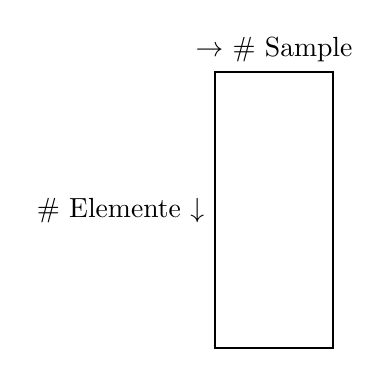
\begin{tikzpicture}
	\node[fill=white,
	thick,
	draw,
	minimum height=3.5cm,
	minimum width=1.5cm
	](n1){};
	\node[left=0cm of n1](t1){\# Elemente $\downarrow$};
	\node[above=0cm of n1](t2){$\rightarrow$ \# Sample};
	\end{tikzpicture}
\end{center}

\#Elemente $>>$ \#samples\\
\begin{itemize}
	\item Genom $\rightarrow$ SNP
	\item Epigenom
	\item \underline{Transkriptom} $\rightarrow$ RNA Content einer Zelle
\end{itemize}

\begin{center}
	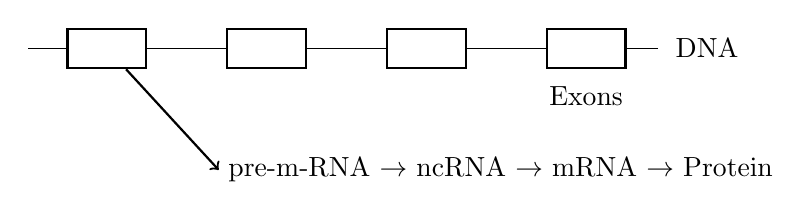
\begin{tikzpicture}
	\node[fill=white,
	thick,
	draw,
	minimum height=0.5cm,
	minimum width=1.0cm,
	](n1){};
	\node[fill=white,
	right=1cm of n1,
	thick,
	draw,
	minimum height=0.5cm,
	minimum width=1.0cm,
	](n2){};
	\node[fill=white,
	right=1cm of n2,
	thick,
	draw,
	minimum height=0.5cm,
	minimum width=1.0cm,
	](n3){};
	\node[fill=white,
	right=1cm of n3,
	thick,
	draw,
	minimum height=0.5cm,
	minimum width=1.0cm,
	](n4){};
	
	\node[below=1cm of n1,xshift=5cm](text1){pre-m-RNA $\rightarrow$ ncRNA $\rightarrow$ mRNA $\rightarrow$ Protein};
	\node[below=0.1cm of n4](text2){Exons};
	\node[right=0.5cm of n4](text3){DNA};
	
	\draw [] (-1,0) edge (n1);
	\draw [] (n1) edge (n2);
	\draw [] (n2) edge (n3);
	\draw [] (n3) edge (n4);
	\draw [] (7,0) edge (n4);
	
	\draw [->,thick] (n1) edge (text1.west);
	
	
	\end{tikzpicture}
\end{center}


\underline{Ziel}: Messen der Werte einer Zielvariablen in Abhängigkeit von unabhängigen Variablen (sog. Kovariaten) \\
\underline{Def}: Ein statistisches Model stellt eine Zielvariable $Y$ in Beziehung zu \underline{einer} oder mehreren Kovariaten (Kovariablen). \\
Zielvariable = Modell(Kovariate) + Fehler \\
\[ Y = f(X) + \epsilon \]
$Y$: Zielvariable oder auch abhängige Variable \\
$X$: Kovariaten oder auch unabhängige Variable \\
$f(X)$: Unbekannte Funktion, die den systematischen Effekt von $X$ auf $Y$ modelliert \\
$\epsilon$: Zufälliger Fehler. Gibt den Anteil der Varianz von $Y$ an, der \underline{nicht} durch $f(X)$ erklärt werden kann. \\
$\Rightarrow$ Statistische Modelle zerlegen die Zielvariable in einen systematischen ($f(X)$) und in einen zufälligen Teil ($\epsilon$). \\

\subsection{Anwendungen von statistischen Modellen}
Inferenz: Ziel ist es die Art des Zusammenhanges zwischen $Y$ und $X$ zu verstehen. Genauer: Wie ändert sich $Y$ als Funktion von $X$?\\
Vorhersage: Ziel ist es, den Wert von $Y$ so genau wie möglich vorherzusagen. Es ist nicht von primären Interesse die (exakte) Form von $f(X)$ zu kennen. \\

\subsection{Schätzen der Funktion $f(X)$}
$f(X)$ wird mittels einer statischen Lernmethode von einer Menge von Trainingsdaten geschätzt. Die geschätzte Funktion wird mit $\hat{f}(X)$ angegeben.
\[ Y = \hat{f}(X) + \epsilon \]
für Trainingsdaten $(X,Y) = \{(x_1,y_1),...,(x_n,y_n)\}\, n$ Beobachtungen.

\subsection{Klassifikation statistischer Lernmethoden}
\underline{Parametrische Methoden}: Für die Funktion $f(X)$ wird eine bestimmte Form angenommen.
\begin{enumerate}
	\item Anzahl der Kovariablen wird vorab festegelegt oder mittels Verfahren der Modellselektion ausgewählt.
	\item Es werden die Gewichte für die Kovariablen geschätzt
\end{enumerate}
Nachteil: 
\begin{enumerate}
	\item weniger flexibel
	\item Gewähltes Modell entspricht oft nicht der wahren Form des Zusammenhanges
\end{enumerate}
Vorteil:
\begin{enumerate}
	\item Da nur Gewichte für Kovariablen gelernt werden müssen, reicht eine geringe Stichprobengröße aus
\end{enumerate}

\underline{Nicht-parametrische Methoden}: Es wird keine bestimmte Form für $f(X)$ vorab angenommen.
Es muß die Form und die Parameter für eine beliebig komplexe Funktion $f(X)$ anhand der Trainingsdaten geschätzt werden. \\
Vorteil:
\begin{enumerate}
	\item Modelle sind sehr flexibel
\end{enumerate}

Nachteil:
\begin{enumerate}
	\item oft weniger gut interpretierbar
	\item oft ein großer Stichprobenumfang notwendig
\end{enumerate}

\section{Lineare Regressionsmodelle}
Als Form für $f(X)$ wird ein (annähernd) linearer Zusammenhang angenommen. Zufallsvariable $Y$ nimmt dabei quantitative Werte an. 
Kovariablen $X_i$ können quantitative oder qualitative Werte annehmen.

\subsection{Einfaches lineares Regressionsmodel}
\underline{Def.} Statistisches Modell, was den Wert der Zielvariablen $Y$ auf Basis der Werte einer einzigen Kovariable $X$, unter der Annahme eines linearen Zusammenhangs modelliert.

\[ Y = \underbrace{\beta_0 + \beta_1}_{Koeffizienten} X + \epsilon \]
$\beta_0$: Mittelwert von $Y$, falls es keinen Zusammenhang gibt, sonst Schnittpunkt mit $y-Achse$. \\
$\beta_1$: \underline{Effekt} der Kovariablen $X$ auf $Y$ an, also den Anstieg in $Y$, wenn $X$ sich um eine Einheit erhöht. (Regressionskoeffizient)\\
$\epsilon$: Fehler $\epsilon \sim N(0,\sigma^2)$ Anteil von $Y$, der nicht durch $\beta_0 + \beta_1 X$ erklärt werden kann.

\subsubsection{Annahmen für zufällige Störgrößen}
\begin{enumerate}
	\item Alle Störungen haben die gleiche Varianz (Homoskedastizität) $Var(\epsilon_i)= \sigma^2$
	\item Alle Störungen sind um 0 verteilt \\ $E(\epsilon_i)=0$ \\ $\Rightarrow$ Einflüsse der Störgrößen heben sich im Mittel auf, d.h. haben keinen systematischen Einflus auf Y
	\item Störgrößen sind unabhängig untereinander: \\ $Cor(\epsilon_i, \epsilon_j) = 0$
\end{enumerate}

\subsubsection{Varianzdekomposition (grafische Darstellung)}
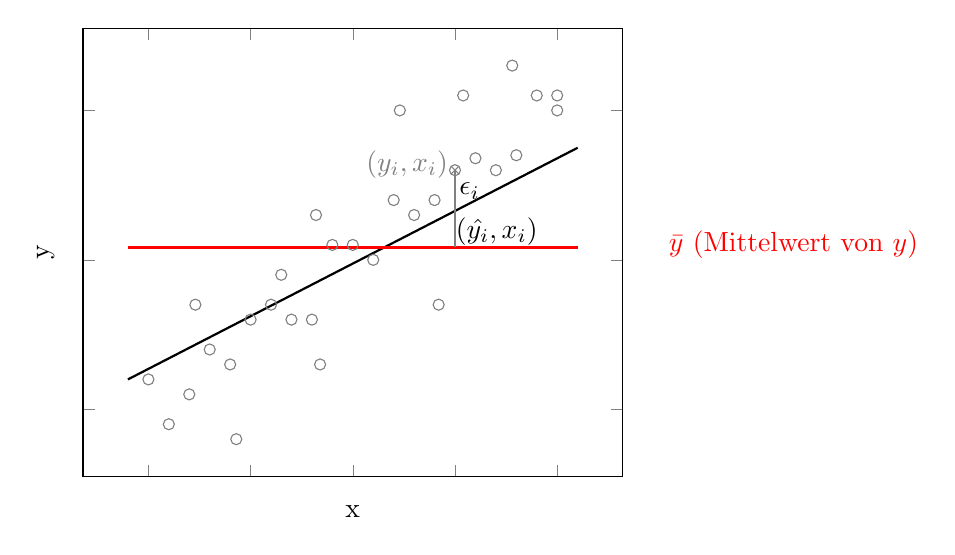
\begin{tikzpicture}
\begin{axis}[%
scatter/classes={%
	a={mark=o,draw=gray},
	b={mark=x, draw=gray}},
xlabel={x},
ylabel={y},
xticklabels={,,},
yticklabels={,,}
]
\addplot[scatter,only marks,%
scatter src=explicit symbolic]%
table[meta=label] {
	x y label
	10 12 a
	11 9 a
	12 11 a
	12.3 17 a
	13 14 a
	14 13 a
	14.3 8 a
	15 16 a
	16 17 a
	16.5 19 a
	17 16 a
	18 16 a
	18.2 23 a
	18.4 13 a
	19 21 a
	20 21 a
	21 20 a
	22 24 a
	22.3 30 a
	23 23 a
	24 24 a
	24.2 17 a
	25 26 a
	25 26 b
	25.4 31 a
	26 26.8 a
	27 26 a
	27.8 33 a
	28 27 a
	29 31 a
	30 30 a
	30 31 a
};
\addplot [thick] coordinates { (9,12) (31,27.5) };
\addplot [thick, red] coordinates { (9,20.83) (31,20.83) };

\addplot [gray] coordinates { (25,20.83) (25,26) };
\end{axis}

\node[red] at (rel axis cs:1.4,0.6){$\bar{y}$ (Mittelwert von $y$)};

\node[] at (rel axis cs:0.85,0.63){$(\hat{y_i},x_i)$};
\node[] at (rel axis cs:0.8,0.72){$\epsilon_i$};
\node[gray] at (rel axis cs:0.684,0.78){$(y_i,x_i)$};

\end{tikzpicture}


\[ \underbrace{\sum\limits_{i=1}^n (y_i - \bar{y})^2}_{\text{TSS (total sum of squares)}} = \underbrace{\sum\limits_{i=1}^n (\hat{y}_i - \bar{y})^2}_{\text{erklärbare Varianz}} + \underbrace{\sum\limits_{i=1}^n (\hat{y}_i - y)^2}_{\text{nicht erklärbare Varianz (RSS)} \epsilon_i = \hat{y}_i -y_i} \]

\subsubsection{Schätzung der Parameter $\beta_0$ und $\beta_1$}
Methode der kleinsten Quadrate: Reduziere Differenz zwischen Werten der Zielvariablen $y_i$ und den vorhergesagten Werten $\hat{y}_i$ für alle Beobachtungen $n$

\[ RSS = \sum\limits_{i=1}^n (y_i -\hat{y}_i)^2 \rightarrow min \]
\[ = \sum\limits_{i=1}^n (y_i -\hat{\beta_0} - \hat{\beta_1} x_i)^2 \rightarrow min \]
\[ \hat{\beta_1} = \frac{\sum\limits_{i=1}^n(x_i - \bar{x})(y_i - \bar{y})}{\sum\limits_{i=1}^n(x_i - \bar{x})} = 
\frac{Cor(X,Y)}{Var(X)} \]
\[ \hat{\beta_0} = \hat{y_i} - \hat{\beta_1}\bar{x} \]
	
%Vorlesung8 14.11.17
\subsubsection{Güte der Schätzungen für $\beta_0$ und $\beta_1$}
Beachten Sie, der wahre Zusammenhang zwischen Y und X ist unbekannt d.h. die wahre Regressionsgerade ist unbekannt. \\
\textbf{Grund:} 
\begin{itemize}
	\item Schätzungen für $\hat{\beta_0}$ und$ \hat{\beta_1}$ hängen von der gewählten Trainingsmenge ab\\
\end{itemize}
\textbf{Daraus Folgt:} 
\begin{itemize}
	\item Die geschätzten Regressionsgeraden schwanken um die wahre Regressionsgerade.
	\item Koeffizienten $\beta_0$ und $\beta_1$ sind Zufallsvariablen, welche auf Basis der gezogengen Beobachtungen $(x_i,y_i)$ geschätzt werden.
\end{itemize}


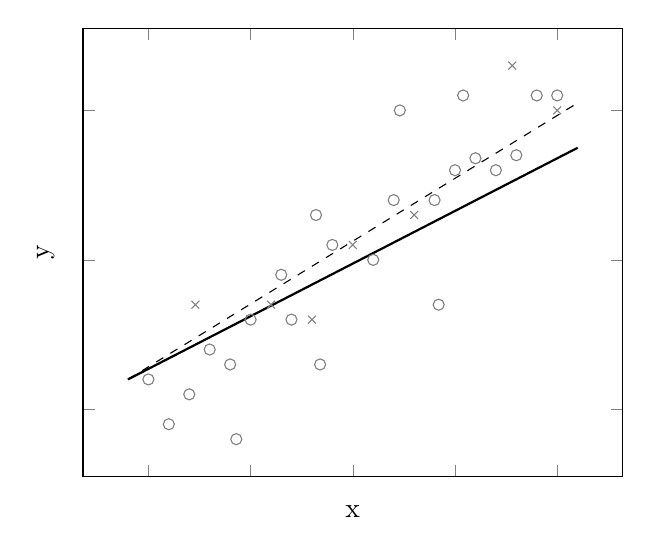
\begin{tikzpicture}
\begin{axis}[%
scatter/classes={%
	a={mark=o,draw=gray},
	b={mark=x,draw=gray}},
xlabel={x},
ylabel={y},
xticklabels={,,},
yticklabels={,,}
]
\addplot[scatter,only marks,%
scatter src=explicit symbolic]%
table[meta=label] {
	x y label
	10 12 a
	11 9 a
	12 11 a
	12.3 17 b
	13 14 a
	14 13 a
	14.3 8 a
	15 16 a
	16 17 b
	16.5 19 a
	17 16 a
	18 16 b
	18.2 23 a
	18.4 13 a
	19 21 a
	20 21 b
	21 20 a
	22 24 a
	22.3 30 a
	23 23 b
	24 24 a
	24.2 17 a
	25 26 a
	25.4 31 a
	26 26.8 a
	27 26 a
	27.8 33 b
	28 27 a
	29 31 a
	30 30 b
	30 31 a
};
\addplot [thick] coordinates { (9,12) (31,27.5) };
\addplot [dashed] coordinates { (9,12) (31,30.5) };
\end{axis}
\end{tikzpicture}




Varianz für $\beta_1$:
\[ 
	Var(\beta_1)= \frac{\sigma_{\epsilon}^2}{\sum\limits_{i=1}^n (x_i-\bar{x})^2} 
\]
mit $\sigma_{\epsilon}^2$ ist die Varianz der Fehler $\epsilon$
\[\sigma_{\epsilon}^2 = \frac{RSS}{n-2} \]

\[\widehat{Var}(\beta_1)=\frac{RSS/(n-2)}{\sum\limits_{i=1}^n (x_i-\bar{x})^2} \]
Varianz von $\beta_1$ ist klein, wenn:
\begin{enumerate}
	\item Varianz der Störgrößen klein ist
	\item Stichprobengrößen n groß ist
\end{enumerate}
\[Var(\beta_0) = \frac{\sigma_\epsilon^2  \sum x_i^{2}}{n Var(X)}\]

\subsubsection{Das Bestimmtheitsmaß $R^2$}
Wie gut ist die Schätzung der Daten anhand der gefitteten Geraden. \\
$\Rightarrow$ Schätzung ist dann besonders gut, wenn der Anteil von RSS an Gesamtvarianz(TSS) klein ist und somit die erklärte Varianz möglichst groß ist.

\[ R^2= \frac{\text{erklärbare Varianz}}{\text{Gesamtvarianz}}
= \frac{TSS-RSS}{TSS} = 1 - \frac{RSS}{TSS}\]
wobei $TSS=\sum(\hat{y}-\bar{y})^2 + RSS$

\[ 0 \leq R^2 \leq 1\]
$R^2 \approx 1$: Ein großer Anteil der Variabilität in der Zielvariablen durch gelernte Regressionsgerade erklärt. \\
$R^2 \approx 0$: \underline{Kein} großer Anteil der Variabilität in der Zielvariablen durch gelernte Regressionsgerade erklärt.

\subsubsection{Testen ob es einen signifikanten Zusammenhang zwischen Y und X gibt}
Frage Existiert irgendein Zusammenhang zwischen X und Y, also $\beta_1 \neq 0$\\
$H_0:$ Es existiert kein Zusammenhang $ \Leftrightarrow $ $ \beta_1 = 0$\\
$H_1:$ Es existiert ein Zusammenhang $ \Leftrightarrow $ $\beta_1 \neq 1$\\

Teststatistik: t-Statistik, welche t-Verteilung folgt $t= \frac{\hat{\beta_1}}{s.d.(\hat{\beta_1})} = \frac{\hat{\beta_1}}{\sqrt{Var(\hat{\beta_1})}} \approx t_{1-\alpha/2, n-2}$

$|t| \leq  t_{1-\alpha/2, n-2} \rightarrow H_0$ wird beibehalten

$|t| >  t_{1-\alpha/2, n-2} \rightarrow H_0$ wird abgelehnt, wir können annehmen das $\beta_1 \neq 0$

\subsection{Multilinerare lineare Regression}
\begin{itemize}
	\item Erweiterung der einfachen linearen Regression auf mehreren Kovariablen $X=\{{X_1, \ldots, X_p}\}$
	\item Identifiziere ein verbessertes Modell als es auf Basis einer einzelnen Kovariable möglich ist 
	\item Individuelle Effekte der Kovariablen $X_I$ können durch partielle Regressionsgeraden modelliert werden.
	\item Jede partielle Regressionsgerade entspricht(modelliert) den Effekt von $X_i$ während alle anderen Kovariablen $X_{j \neq i}$ ihren Mittelwert annehmen
\end{itemize}

\subsubsection{Additives multivariables lineares Regressionsmodell}
Annahme: Effekt einer Kovariablen $X_i$ auf Y ist unabhängig von allen anderen Kovariablen 
\[Y = \beta_0 + \beta_1X_1 + \beta_2X_2 + \ldots + \beta_p X_p + \epsilon\]
$ \beta_1,\ldots,\beta_p$ geben Effekte der Kovariablen $X_1, \ldots, X_p$ auf Y an.\\
p: Anzahl der Kovariablen\\ 
$ \beta_0 $ Mittelwert von Y , falls alle Koeffizienten $ \beta_j = 0 $\\
$\epsilon$ ist der Fehler $\epsilon \sim N(0, \sigma^2)$


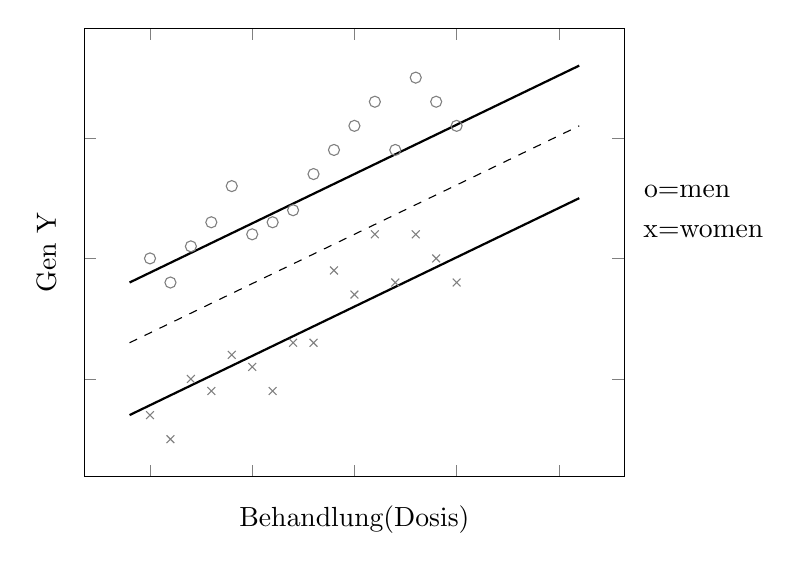
\begin{tikzpicture}
\begin{axis}[%
scatter/classes={%
	a={mark=o,draw=gray},
	b={mark=x,draw=gray}},
ylabel={Gen Y},
xlabel={Behandlung(Dosis)},
xticklabels={,,},
yticklabels={,,}
]
\addplot[scatter,only marks,%
scatter src=explicit symbolic]%
table[meta=label] {
	x y label
	10 20 a
	11 18 a
	12 21 a
	13 23 a
	14 26 a
	15 22 a
	16 23 a
	17 24 a
	18 27 a
	19 29 a
	20 31 a
	21 33 a
	22 29 a
	23 35 a
	24 33 a
	25 31 a
	10 7 b
	11 5 b
	12 10 b
	13 9 b
	14 12 b
	15 11 b
	16 9 b
	17 13 b
	18 13 b
	19 19 b
	20 17 b
	21 22 b
	22 18 b
	23 22 b
	24 20 b
	25 18 b
};
\addplot [thick] coordinates { (9,7) (31,25) };
\addplot [thick] coordinates { (9,18) (31,36) };
\addplot [dashed] coordinates { (9,13) (31,31) };
\end{axis}
\node[] at (rel axis cs:1.23,0.63){x=women};
\node[] at (rel axis cs:1.2,0.72){o=men};
\end{tikzpicture}
\todo{Hoher Fehler mit einfacher Regression (gestrichelt), also additiv nutzen}



\subsubsection{Multiplikatives Modell}
\begin{itemize}
	\item Interaktionen zwischen den Kovariablen sind möglich
	\item D.h. partieller Effekt einer Kovariablen $X_i$ kann vom partiellen Effekt von $X_j$ abhängig sein
\end{itemize}
\[Y = \beta_0+ \beta_1X_1 + \beta_2X_2 + \beta_3 X_1X_2 + \beta_4 X_3 +\ldots \beta_{p+1}X_p + \epsilon\]

$\beta_3:$ Gibt an, inwieweit der Effekt von $X_1$ von den Werten von $X_2$ abhängt

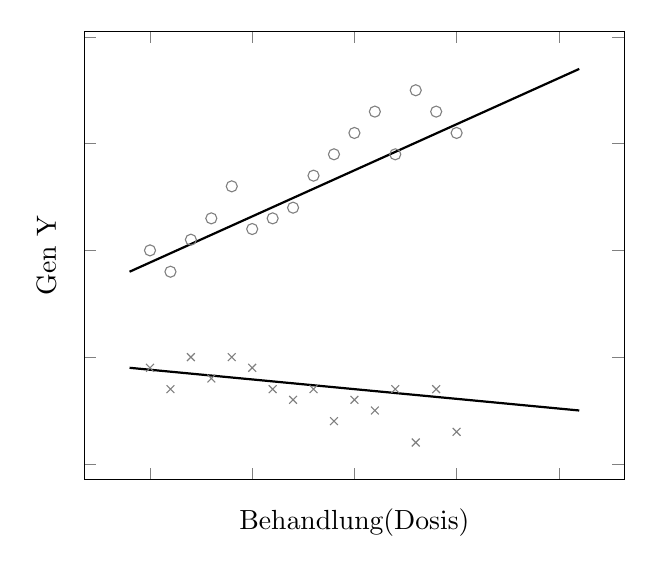
\begin{tikzpicture}
\begin{axis}[%
scatter/classes={%
	a={mark=o,draw=gray},
	b={mark=x,draw=gray}},
ylabel={Gen Y},
xlabel={Behandlung(Dosis)},
xticklabels={,,},
yticklabels={,,}
]
\addplot[scatter,only marks,%
scatter src=explicit symbolic]%
table[meta=label] {
	x y label
	10 20 a
	11 18 a
	12 21 a
	13 23 a
	14 26 a
	15 22 a
	16 23 a
	17 24 a
	18 27 a
	19 29 a
	20 31 a
	21 33 a
	22 29 a
	23 35 a
	24 33 a
	25 31 a
	10 9 b
	11 7 b
	12 10 b
	13 8 b
	14 10 b
	15 9 b
	16 7 b
	17 6 b
	18 7 b
	19 4 b
	20 6 b
	21 5 b
	22 7 b
	23 2 b
	24 7 b
	25 3 b
};
\addplot [thick] coordinates { (9,9) (31,5) };
\addplot [thick] coordinates { (9,18) (31,37) };
\end{axis}
\end{tikzpicture}


\subsubsection{Schätzung der Koeffizienten $\beta_1 ... \beta_p$}
Methode der kleinsten Quadrate
\[\hat{Y} = \hat{\beta_0} + \hat{\beta_1} X_1 + ... + \hat{\beta_p} X_p \]

\[ RSS = Var(\epsilon)= \sum\limits_{i=1}^n (y_i - \hat{y_i} )^2 \]
\[ \sum (y_i - \hat{\beta_0} - \hat{\beta_1} X_1 - ... - \hat{\beta_p} X_p )^2 \rightarrow min \]
Über partielle Ableitungen werden die Koeffizienten $\beta_i$ geschätzt


%Vorlesung vom 14.12.17
%\section{Fortsetzung lineare Regressionsmodelle}
\section{Wichtige Fragen}
\textbf{1.Frage}: Ob es einen Zusammenhang zwischen $X_i$ und $Y$ gibt? \\
\textbf{2.Frage}: Welche Kovariablen haben einen Effekt auf $Y$? \\
\textbf{3.Frage}: Wie gut repräsentiert das multivariate Regressionsmodell die beobachtete Varianz von $Y$?\\

\subsection{Gibt es einen Zusammenhang} F-Test\\
Beantwortet: Hat mindestens eine der Kovariablen einen Effekt.
\[ H_0: \beta_1=\beta_2=\dots=\beta_p=0 \]
\[ H_1: \beta_j \neq 0 \]
\[F= \frac{\text{erklärte Varianz}}{\text{unerklärte Varianz}} = \frac{\frac{TSS - RSS}{p}}{\frac{RSS}{n-p-1}} \]
\begin{itemize}
	\item $H_0$ kann nicht abgelehnt werden, wenn $F \sim 1$
	\item $H_1$ kann abgelehnt werden, wenn $F > 1$
\end{itemize}

\subsection{Welche der Kovariablen haben einen Effekt}
Jede einzelne Koeffizient $\beta_1,\dots,\beta_p$ kann mittels einen t-Tests getestet werden:
\[ H_0: \beta_j = 0 \]
\[H_1: \beta_j \neq 0 \]
\[ t= \frac{\hat{\beta_j}}{sd(\beta_j)} \]
adjustierte p-Werte: \\
$\Rightarrow$ Bonferroni-Korrektur
$\Rightarrow$ Benjamin-Hochberg

\subsection{Güte des Fits}
\[ R^{2} = \frac{\text{erklärte Varianz}}{\text{unerklärte Varianz}} = \frac{TSS -RSS}{TSS} \]
\[ \text{adjustiertes} R_{adj}^{2} = 1 - \frac{\frac{TSS - RSS}{p}}{\frac{RSS}{n-p-1}} \]

\section{Qualitative Kovariablen}
In Genexpressionsanalysen ist man oft daran interessiert, den Effekt von kategorialen Variablen zu untersuchen.\\
$\Rightarrow$ Kategoriale und quantitative Variablen können im selben Modell aufgenommen werden \\
$\Rightarrow$ Kategoriale Variablen werden mittels sog. Dummy-Variablen kodiert:
	\begin{itemize}
		\item \#Kategorien = 2 $\Rightarrow$ als binäre Variable kodiert
		\item \#Kategorien $>$ 2 $\Rightarrow$ meherere binäre Variablen
	\end{itemize}

\subsection{Treatment-Contrast Parametrisierung}
\[ X_i = \begin{cases}
		1, i \hat{=} \text{ level 1 (female)} \\
		0, i \hat{=} \text{ level 2 (male)}
\end{cases} \]

\[ Y = \begin{cases}
		\beta_0 + \beta_1 + \epsilon, \text{ falls } i = \text{ level 1 } \\
		\beta_0 + \epsilon, \text{ falls } i = \text{ level 2 } \\
\end{cases} \]

$\beta_0:$ Mittlerer Effekt von level 2\\
$\beta_1:$ Mittlere Differenz zwischen level 1 und level 2\\

\subsection{Group-Means-Parametrisierung}
\[ X_i = \begin{cases}
		1, i \hat{=} \text{ level 1 (female)} \\
		-1, i \hat{=} \text{ level 2 (male)}
\end{cases} \]

\[ Y = \begin{cases}
		\beta_0 + \beta_1 + \epsilon, \text{ falls } i = \text{ level 1 } \\
		\beta_0 - \beta_1 + \epsilon, \text{ falls } i = \text{ level 2 } \\
\end{cases} \]
$\beta_0:$ Mittlerer Effekt (unabhängig vom gewählten Level)\\
$\beta_1:$ Anteil den Level 1 größer als der mitlere Effekt ist bzw. den Anteil von Level 2, der kleiner als der mittlere Effekt ist\\

\section{Annahmen für lineare Regressionsmodelle}
\begin{enumerate}
	\item Zusammenhang ist (annähernd linear)
	\item Kovariablen sind unabhängig (keine Kolinearität)
	\item Fehlerterme haben eine konstante Varianz $\epsilon_i \sim N(0, \sigma^{2} )$ (Homoskedastizität)
\end{enumerate}
$\Rightarrow$ Diagnostik für lineare Modelle

\subsection{Test auf Nonlinearität}
$\Rightarrow$ Residualplot
$\Rightarrow$ Dieser sollte keine Muster in der Punktwolke erkennen lassen. Denn bei linearem Zusammenhang sollten die Residuen zufällig um vorhergesagten Werte $\hat{y_i}$ streuen

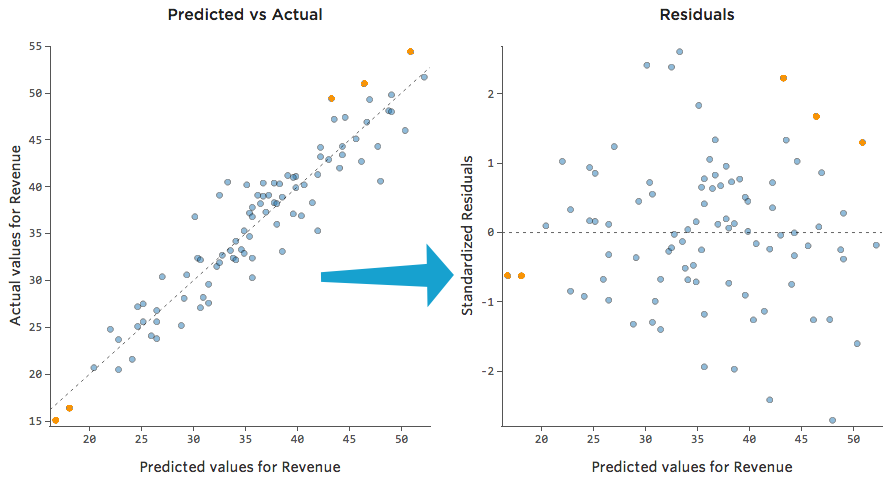
\includegraphics[scale=0.4]{VorlesungenTexDateien/images/residual}
\todo{Kein Muster erkennbar}
       
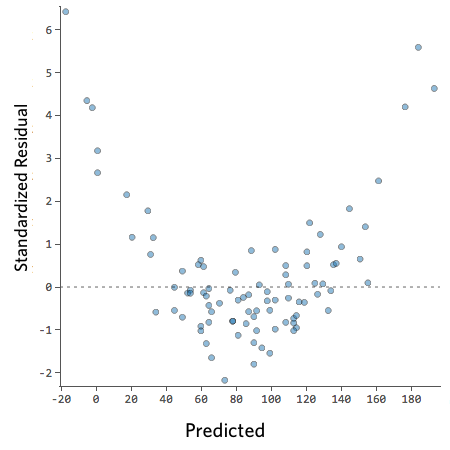
\includegraphics[scale=0.5]{VorlesungenTexDateien/images/Nonlinear-residual-11}
\todo{Nonlinearer Zusammenhang erkennbar}

\subsection{Test auf Kollinearität}
Kollinearität wird beobachtet, falls 2 oder meherere Variablen linear abhängig voneinander sind.

\[ X_i = \lambda_0 + \lambda_1 X_i \]

Variance Inflation Faktor (VIF):
\[ VIF(\hat{\beta_j})= \frac{1}{1- R_{X_j|X_{p \neq j}}^{2}} \]
\[ R_{X_j|X_{p \neq j}}^{2} \sim 1 \Rightarrow VIF >> 1 \]

\paragraph{Probleme bei Kollinearität}
\begin{enumerate}
	\item Es ist nicht möglich den Effekt den die abhängigen Kovariablen auf  haben voneinander zu trennen
	\item $sd(\hat{\beta_i})$ ist erhöht, denn: 
		\begin{itemize}
			\item Annahme für $\beta_i$: gibt den Effekt von $X_i$ auf $Y$ an $\Leftrightarrow$ alle anderen Kovariablen konstant sind
			\item Falls aber $X_i$ und $X_j$ linear abhängig sind, dann gibt es viele Wertepaare von $\beta_i$ und $\beta_j$, die nun einen ähnlichen Fehler (RSS) haben
		\end{itemize}
		$\Rightarrow$ Schätzer $\hat{\beta_i}$ und $\hat{\beta_j}$ sind ungenauer \\
		$\Rightarrow$ geringere Power für t-Test
\end{enumerate}

\paragraph{Wie kann mit Kollinearität umgegangen werden?}
\begin{enumerate}
	\item Entferne alle bis auf eine der linear abhängigen Kovariablen
	\item Fasse linear abhängige Kovariablen in einer neuen Kovariablen zusammen z.B. durch Bildung des Mittelwertes \\
		Beachte: Es kann notwendig sein, diese Kovariablen vorher zu standardisieren
\end{enumerate}

\subsection{Test auf Heteroskedastizität}
Homoskedastizität ist gegeben, falls Fehlerterme $\epsilon_i$ eine konstante Varianz
\[ Var(\epsilon_i) = \sigma_{\epsilon}^{2} \text{ für alle  Beobachtungen } (x_i, y_i) \] 
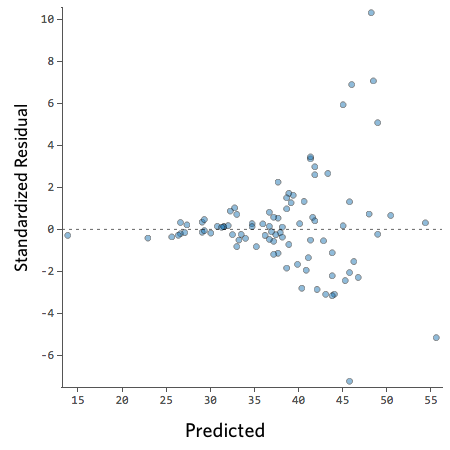
\includegraphics[scale=0.5]{VorlesungenTexDateien/images/Heteroscadicity}
\todo{Trichterform $\Rightarrow$ Heteroskedastizität}

\paragraph{Wie wird mit Heteroskedastizität umgegangen}
\begin{enumerate}
	\item Stabilisieren der Varianz der Fehler:\\
		Werte für $Y$ so transformiert werden, dass größere Werte kleinere Werte annehmen:
		\begin{enumerate}
			\item $log(Y)$
			\item $glog(Y) = log_{2}(\frac{1}{2} y + \frac{1}{2}\sqrt{y^{2} + a^{2}} ) $ \\
				$\Rightarrow$ Interpoliert $y$-Werte zwischen $log_2(Y)$ für große Werte von $Y$ und für kleine $\frac{y}{a} + log_2(\frac{a}{2})$
		\end{enumerate}
	\item Schätzen der Koeffizienten \(\beta\); mittels gewichteter Methode der kleinsten Quadrate
		\[ RSS := \sum_{i=1}^{n}(y_i - \hat{y}_i)^2 \rightarrow \min \]
		Bei klassischen Methode der kleinsten Quadrate erhält jede Beobachtung das gleiche Gewicht.
		Gewichtete Methode der kleinsten Quadrate:

		\[ RSS = \sum_{i = 1}^{n}\omega_i (y_i - \widehat{y_i})^2 \]
		\[ \omega_i = \dfrac{1}{\hat{Var}(y_i)} \]
		das bedeutet Alle Beobachtungen \(y_i\) mit einer höheren Varianz erhalten ein geringeres Gewicht \(\omega_i\) als Beobachtungen mit einer geringeren Varianz.  
	\item Verwendung von Generalisierten linearen Modellen
\end{enumerate}

\section{Generalisierte lineare Modelle (GLM)}
Verallgemeinerung der Theorie für lineare Modelle

Herleitung anhand linearer Regressionsmodelle
unter der Annahme, dass bei linearen Regressionsmodellen der Fehler \( \epsilon_i\) normalverteilt sind \((\epsilon_i \approx N(0, \sigma^2))\) kann die lineare Regression für

\[ Y = \beta_0 + \beta_1 X + \epsilon \]
auch wie folgt dargestellt werden

\begin{align*}
E(Y|X) &= E(\beta_0 + \beta_1 X + \epsilon)\\
&=  E(\beta_0) + E(\beta_1) X + E(\epsilon)\\
&= \beta_0 + \beta_1 X + 0\\
E(Y|X) &= g^{-1} (\beta_o + \beta_1 + X)
\end{align*}

Die beliebige Funktion \(g^{-1}\) modelliert die Streuung der Beobachtungen \( y_i\) um die geschätzten Werte \(\hat{y_i}\). \\
Daher muss für GLMs keine Konstante Varianz für Fehler \(\epsilon_i\) vorausgesetzt werden
\[
g(E(y|X)) = \beta_0 + \beta_1 X
\]
\(g(E(y|X))\) wird als Link-Funktion bezeichnet.
Die Link-Funktion definiert die Bezeichnung zwischen dem linearen Term \(\beta_0+ \beta_1 X\) und der bedingten Erwartung von \(Y\) gegeben \(X E(Y|X)\)

\subsubsection*{Definition für GLMs}
Sie bestehe aus 3 Komponenten 
\begin{enumerate}
	\item Zufallskomponente: Definiert die Verteilung von Y. 
	Die Verteilung kommt aus der Familie der Exponentialverteilungen	
	\[
	\underbrace{f(y | \theta, \phi)}_{g()} = \exp\{\frac{y\theta- b\theta}{a(\phi)} + c(y, \phi)\}
	\]
	\begin{itemize}
		\item [] \(\theta\) bzw. g(): Transformation des Erwartungswertes für Y
		\item [] \(\phi\): Streuungsparamter, Dispersion
		\item [] \(a(),b(), c()\): Spezifische Funktion je nach Typ der gewählten Exponentialverteilung
		
	\end{itemize}

	\item linearer Term Y:
	Linearer Term, welcher die Kovariablen im GLM definiert
	\begin{align*}
		&\beta_0 +\beta_1 X \\
		&\beta_0 + \beta_1 X_1 + \ldots + \beta_p X_p
	\end{align*}
	
	\item Link Funktion:
	Die Link-Funktion \(\theta\)(oder g()) definiert die Beziehung zwischen dem linearen Term und der bedingten Erwartung E(Y|X)
\end{enumerate}

Beispiel:
\begin{tabbing}
	\hspace{0.25\linewidth}\=\hspace{0.25\linewidth}\=\hspace{0.25\linewidth}\=\kill
	\textbf{Modell}	\>  \textbf{abhängige Variable}\>  \textbf{Vert. d. Residuen}\> \textbf{Link Funktion}\\ 
	lineare Regression\>  qualitativ, stetig\>  normal verteilt\> \(g(E(Y|X)) = E(Y)\)\\ 
	logistische Regression\>  binär\>  binomial verteilt\> \(g(E(Y|X)) = \log(\frac{E(Y)}{1-E(Y)}) \)\\ 
	log.-lin. Regression\>  diskret \>  poisson verteilt\> \(g(E(Y|X)) = \log(E(Y))\)\\
\end{tabbing} 

Dichtefunktion der Normalverteilung in die generalisierte Form der Exponentialverteilungen übertragbar\\

generalisierte Form für Exponentialverteilungen :
\[
f(y| \theta, \phi) = \exp(\frac{y\theta - b(\theta)}{a(\phi)} + c(y,\phi))
\]
Dichtefunktion für die Normalverteilung

\begin{align*}
	f(y| \mu , \sigma^2) &= \frac{1}{\sqrt{2\pi \sigma^2}} \exp(- \frac{(y-\mu)^2}{2\sigma^2}) = \frac{1}{a} e^b = a^{-1} e^b = e^{-ln a} e^b = e^{-\ln a + b}\\
	&= \exp (-ln \sqrt{2\pi \sigma^2} - \frac{(y-\mu)^2}{1\sigma^2})\\
	&= \exp (-\frac{y^2 - 2y\mu + \mu^2}{2 \sigma^2})
	- \ln(\sqrt{2\pi \sigma^2}) \\
	&= \exp\frac{- y^2 + 2y\mu - \mu^2}{2 \sigma^2} - ln(\sqrt{2\pi \sigma^2})\\
	&= \exp\frac{ 2y\mu - \mu^2}{2 \sigma^2}- \frac{y^2}{2\sigma^2} - ln(\sqrt{2\pi \sigma^2})\\
	&= \exp \underbrace{\frac{ y \mu - \frac{\mu^2}{2}}{\sigma^2}}_{c(\phi)} - 
	\underbrace{\frac{y^2}{2\sigma^2} - ln(\sqrt{2\pi \sigma^2})}_{c(y, \phi)}
\end{align*}

mit \\
\tab  $\theta= g() = \mu = E(Y|X)$\\
\tab $b(\theta) = \frac{\mu^2}{2}$\\
\tab $a(\phi) = \sigma^2$ = Streuungsparamter für Normalverteilung \\




\subsection{Schätzen der Parameter für GLMs}
Neben den Koeffizienten $\beta_i$ der linearen Link Funktion muss auch der Dispensionsparameter $\phi$ geschätzt werden. 
Dafür werden oft Maximum likelihood Methoden verwendet

\subsubsection*{Maximum likelihood Methoden (MLE)}
Schätzwert $\hat{\theta}$ für einen beliebigen Parameter $\theta$ wird so gewählt, dass die  likelihood Funktion $L(\theta|x_1, \ldots, x_n)$ für $ n $ Beobachtungen ihr Maximum erreicht.
Sind die Beobachtungen $x_i$ unabhängig, wird die Likelihoodfunktion wie folgt definiert:

\[
L(\theta|x_1, \ldots, x_n)  = \prod_{i=1}^{n} f(x_i|\theta)
\]
$f(x_i|\theta)$: Dichtefunktion für Zufallsvariable X mit Beobachtungen $x_1$, $\ldots$ , $x_n$\\

Daher ist die likelihood Funktion  $L(\theta|x_1, \ldots, x_n)$ eine Funktion des unbekannten Parameter $\theta$ gegeben der Beobachtungen $x_1, \ldots, x_n$. Sie gibt die Werte für den Parameter $\theta$ an, die gegeben der Beobachtungen $x_1,\ldots, x_n$ am wahrscheinlichsten sind.

\[
\log (L(\theta|x_1, \ldots, x_n))  = \sum_{i=1}^{n} \log(f(x_i|\theta))
\]
Als Schätzer für $\theta$ rechnet man den sogenannten Maximun Likelihood Schätzer aus: $\hat{\theta}_{ML}$

$\hat{\theta}_{ML}$ ist der Wert unter dem die Likelihoodfunktion ihr Maximum erreicht.
\[
\frac{\partial L}{\partial \theta} = 0 \text{\tab z.B durch Newton-Verfahren}
\]


\begin{itemize}
	\item[$\rightarrow$] Methode der kleinsten Quadrate ist eine Sonderform für ML-Methoden
	\item[$\rightarrow$] ML Schätzer für Parameter der Normalverteilung sind 
\end{itemize}


\[\mu = \frac{1}{n} \sum_{i = 1}^{n} x_i \]
\[\sigma^2 = \frac{1}{n} \sum_{i = 1}^{n}(x_i - \bar{x})^2\]

%Vorlesung vom 04.01.18
\subsection{Schätzen der Kovariablen mittels MLE (GLMs)}
Die log-likelihood für n unabhängige Beobachtungen $y_1,\cdots,y_n$ direkt aus der generalisierenden Form der Exponentioalverteilung erstellen:
\[ l(y|\theta, \phi) = \exp \left( \frac{y \theta - b(\theta)}{a(\phi)} + c(y,\phi) \right) \]
\[ log l (\theta, \phi, y) = \sum\limits_{i=1}^{n} log l (y_i | \theta, \phi) = \sum\limits_{i=1}^{n} \left( \frac{y \theta - b(\theta)}{a(\phi)} + c(y,\phi) \right) \]
\[\theta_i = g(\mu_i)=\beta_0 + \beta_1 X_1,\dots,\beta_n X_n \]
$\Rightarrow$ Partielle Ableitungen der likelihood Funktion für einzelnen Regressionskoeffizienten berechnet

\section{Test auf signifikanten Effekt}
\begin{enumerate}
	\item Wald-Test
	\item Likelihood-Ratio-Test
\end{enumerate}

\subsection{Wald-Test}
Der Wald-Test ist eine generalisierte Form des t-tests. Hier ist der Wert der Teststatistik standardnormalverteilt $(\sim N(0,1))$.
\[Z_n = \frac{\bar{X} - \mu}{\sigma / \sqrt{n}} \]
Ein Maximum-likelihood-Schätzer kann als Mittelwert aus einer Summe einer großen Anzahl von Zufallsvariablen interpretiert werden.
Bei großen n die Summe von identisch verteilten und unabhängigen Zufallsvariablen asymptotisch normalverteilt ist (zentraler Grenzwertsatz).
\[\sum\limits_{i=1}^{n} X_i \sim N(n \cdot \mu, n \cdot \sigma^{2}) \]
Aus dem zentralen Grenzwertsatz folgt, dass die Mittelwerte von beliebig verteilten Zufallsvariablen standardnormalverteilt sind. \\
$\Rightarrow$ Kann für einen Ml-Schätzer der Wald-Test genommen werde, um den Wert des Schätzers mit dem Wert aus einer Grundgesamtheit abzugleichen

\[ H_0: \beta_i = 0 \]
\[ H_1: \beta_i \neq 0 \]
\[ w = \frac{\hat{\beta}_{iML}-0}{\sigma / \sqrt{n}} \sim N(0,1) \]
\[ w = \frac{\hat{\beta}_{iML}^{2}-0}{Var(\sigma / \sqrt{n})} \sim \chi_{df,1-\alpha}^{2} \]
\todo{ML im Index heißt der Koeffizient wurde mit Maximum Likelihood geschätzt. df im Index heißt degrees of freedom}
$\Rightarrow$ Da ML-Schätzer nur bei großen n standardnormalverteilt sind, ist der Wald-Test nur bei großen n zulässig \\
$\Rightarrow$ Wald-Test approximiert einen Likelihood-Ratio Test \\
$\Rightarrow$ Im Vergleich zum LR-Test muß nur ein Modell (mit allen Koeffizienten) gefittet werden \\
\subsection{LR-Test}
Vergleicht die likelihood des gesamten Modells mit der Likelihood des reduzierten Modells. Das reduzierte enthält den Koeffizienten, der getestet werden soll nicht.
\[ H_0 : \beta_i = 0 \Leftrightarrow g(\mu) = \beta_0 \]
\[ H_0 : \beta_i \neq 0 \Leftrightarrow g(\mu) = \beta_0 + \beta_1 X \]

\[LR = \frac{l(H_0 | x_1,\cdots,x_n}{l(H_1 | x_1,\cdots,x_n}\]
\[ -2 ln LR \sim  \chi_{df,1-\alpha}^{2} \]
$\Rightarrow$ LR-Test erfordert, dass beide Modelle $g(\mu)=\beta_0$ und $g(\mu)=\beta_0 + \beta_1 X$ gefittet werden müssen.
$\Rightarrow$ LR-Test st allerdings auch für geringe Stichprobengrößen geeignet. (Im Vergleich zum Wald-Test)



%Vorlesung 9 16.11.2017
\section{Nichtlineare Regression}
%\subsection{Rückblick: Lineare Regression}
%\[ Y= \beta_0 + \beta_1 x_1^{(1)} + ... + \beta_k x_i^{(k)} + \epsilon_i, \; i \in \{1,...,n\} \]
%\begin{itemize}
% \item $n$: Anzahl Messungen 
% \item $k$: Anzahl Kovariablen 
% \item $x_i^{(j)}$: Wert der Kovariablen $j$ von Individuum $i$
% \item $\epsilon_i$: zufällige Störungshäufigkeit $\epsilon_i \sim N(0, \sigma^2), \sigma^2 > 0$, unabh.
% \item $\beta_j$: unbekannter, wahrer, zu schätzender Parameter
%\end{itemize}
%$\rightarrow$ Kleinste Quadrate Methode:
%\[ \sum\limits_{i=1}^n \left(y_i - (\beta_0 + \beta_1 x_1^{(1)} + ... + \beta_k x_i^{(k)} \right)^2 \rightarrow min \]

\begin{itemize}
 \item häufig nichtlineare Zusammenhänge zwischen abhängiger und unabhängigen Variablen 
	\begin{sloppypar}
	 $\rightarrow$ manchmal aus dem theoretischen Wissen/empirischen Beobachtungen bekannt
	\end{sloppypar}
 \item beschränkter Wertebereich, z.B. $R=[0,1]$ (Wahrscheinlichkeit an einer Krankheit zu erkranken)
 \item diskreter Wertebereich, z.B. $R={0,1}$ (dichotome Zielgröße ``Ja/Nein'')
\end{itemize}

\begin{tikzpicture}
\begin{axis}[%
scatter/classes={%
	a={mark=o,draw=gray}},
xlabel={x},
ylabel={y},
xticklabels={,,},
yticklabels={,,}
]
\addplot[scatter,only marks,%
scatter src=explicit symbolic]%
table[meta=label] {
	x y label
	5 12 a
	6 14 a
	7 16 a
	8 17 a
	9 18 a
	10 18 a
	11 17.5 a
	12 17 a
	13 16 a
	
	15 16 a
	16 18 a
	17 20 a
	18 21 a
	19 22 a
	20 22 a
	21 21 a
	22 20 a
	23 19 a
	
};
\addplot [thick] coordinates { (4,14) (23,21) };
\end{axis}
\end{tikzpicture}
\todo{Man sieht Lineare Regression ist hier schlecht}
\subsection{Modell}
\[Y_i = \underbrace{h}_{\text{Funktion i.A. nichtlinear}} \left(\underbrace{x_i^{(1)},...,x_i^{(k)}}_{\text{Kovariablen}};
\underbrace{\theta_1,...,\theta_p}_{\text{(unbekannte Parameter)}} \right) + \epsilon_i, \; i \in \{1,...,n\} \]

$\epsilon_i \sim N(0,\sigma^2) , \sigma^2 >0$, unabhängig

\subsubsection{Beispiele}
Biochemischer Sauerstoffverbrauch von Mikroorganismen
\[h(x;\theta_1,\theta_2) = \theta_1(1-exp(-\theta_2 x)) \]

Cobb-Douglas-Funktion
\[h(x^{(1)},x^{(2)}; \theta_1, \theta_2, \theta_3)= \theta_1(x^{(1)})^{\theta_2} (x^{(2)})^{\theta_3} \]

Polynomiale Regression
\[h(x; \theta_0,..., \theta_p)= \theta_0 + \theta_1 x  + \theta_2 x^2 + ... + \theta_p x^p \]

prinzipiell ``alles möglich'' \\

Wahl/Entscheidung anhand des Wissens über das Problem

\subsection{Linearisierung}
manchmal lässt sich $h$ in einen Ausdruck verwandeln, welcher linear in den transformierten Variablen ist \\
$\rightarrow$ lineare Regression \\
\underline{Beispiel:}
\[ h(x; \theta_1, \theta_2) = \theta_1 x^{\theta_2} \]

\[ \Rightarrow \underbrace{\log h}_{=:  \tilde{h}}(x; \theta_1, \theta_2) = \log \theta_1 + \log x^{\theta_2} \]
\[= \underbrace{\log \theta_1}_{=: \tilde{\theta}_1} + \underbrace{\theta_2}_{=: \tilde{\theta}_2} \underbrace{ \log x }_{=: \tilde{x}} \]
\[ \rightarrow \tilde{h}(\tilde{x};\tilde{\theta}_1 \tilde{\theta}_2 ) = \tilde{\theta}_1 \tilde{\theta}_2 \tilde{x} \]
Lineare Regression
\[ Y_i=\log y_i \]
\[ \rightarrow \tilde{Y_i} = \log y_i = \tilde{h}(\tilde{x}_i \tilde{\theta}_1 \tilde{\theta}_2) + \epsilon_i \]
\[ \tilde{\theta}_1 + \tilde{\theta}_2 \tilde{x}_i + \epsilon_i, \; i \in \{1,...,n\} \]
$\rightarrow$ Schätzung von $\tilde{\theta}_1$ und $\tilde{\theta}_2$ \\
Aber: $\epsilon_i \sim N(0,\sigma^2), \sigma^2 > 0$, unabh.\\
Rücktransformation:
\[ Y_i = \exp(\tilde{\theta}_1 + \tilde{\theta}_2 \tilde{x}_i + \epsilon_i ) \]
\[ = \underbrace{\exp(\tilde{\theta}_1)}_{=\theta_1} \underbrace{\exp(\tilde{\theta}_2\tilde{x}_i)}_{
	\substack{= \exp(\theta_2 x_i) \\ = \exp ( \exp ( \tilde{x}_i ))^{\theta_2} \\ = x_i^{\theta_2} }}
\exp(\epsilon_i) \]
\[= \theta_1 x_i^{\theta_2} \exp (\epsilon_i) \]

$\rightarrow$ Durch Transformation betrachtet man ein Modell, in dem sich die Fehler
\begin{itemize}
 \item multiplikativ verhalten
 \item log - normalverteilt sind
\end{itemize}

\[``X \sim LN`` \text{ , falls } `` \log (x) \sim N `` \]

\underline{Vergleich:}
\[ Y_i= \theta_1 x_i^{\theta_2} + \epsilon_i , \; i \in \{1,...,n\} \text{ mit } \epsilon_i \sim N(0, \sigma^2), \sigma^2 > 0 \text{, unabhängig} \]

Linearisierung nur, falls sich die Fehler tatsächlich so wie in der transformierten Variable verhalten \\
$\Rightarrow$ Residuenanalyse

\subsection{Spezielle nichtlineare Situation}

\[Y_i = \underbrace{
\sum_{j=1}^{p} \theta_j h_j (x^{(1)},...,x^{(k)} )}
_{\mathrel{\widehat{=}}  h (x_i^{(1)},...,x_i^{(k)}; \theta_1,..., \theta_p) }
+ \epsilon_i , \; i \in \{1,...,n\} \]

\underline{Beispiele:}
\begin{enumerate} 
 \item $h_j((x_i^{(1)},...,x_i^{(k)}) = x_i^{(j)} \rightarrow$  lineares Modell
 \item $h_j(x_i) = x_i^{j} \rightarrow$ polynomielle Terme
 \item $h_j((x_i^{(1)},...,x_i^{(k)}) = \mathbbm{1}_{[\alpha_j,\alpha_{j+1})} (x_i^{(j)})$ \todo{$\mathbbm{1}$ ist Indikatorfunktion}\\
 $= \begin{cases}
 1, \text{ falls } x_i^{(j)} \in [\alpha_j,\alpha_{j+1}) \\
 0, \text{ falls } x_i^{(j)} \notin [\alpha_j,\alpha_{j+1}) \\
 \end{cases}$
\end{enumerate}

\subsubsection{Polynomiale Regression (Hier:k=1)}
\[Y_i = \theta_0 + \theta_1 x_i^1 +  \theta_2 x_i^2 + ... +  \theta_p x_i^p + \epsilon_i, \; i \in \{1,...,n\} \]

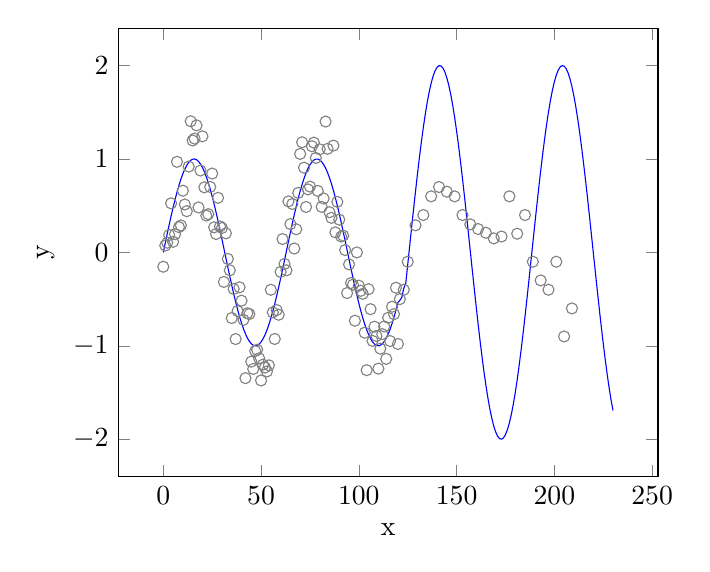
\begin{tikzpicture}
\begin{axis}[%
scatter/classes={%
	a={mark=o,draw=gray}},
xlabel={x},
ylabel={y}
%,
%xticklabels={,,},
%yticklabels={,,}
]
\addplot[scatter,only marks,%
scatter src=explicit symbolic]%
table[meta=label] {
	x y label
0 -0.153598481556401  a
1 0.073583842847978  a
2 0.10389364452171  a
3 0.186267113992389  a
4 0.52527384219649  a
5 0.112936649511624  a
6 0.195148680164532  a
7 0.969726716445442  a
8 0.270429246127571  a
9 0.288292071765007  a
10 0.660444693472895  a
11 0.512673438624097  a
12 0.441350472118466  a
13 0.918543608896422  a
14 1.40390367343846  a
15 1.19766597575237  a
16 1.21809212723937  a
17 1.35964192321696  a
18 0.480920001610398  a
19 0.876400165916276  a
20 1.24273100042559  a
21 0.69634472843208  a
22 0.393930384502455  a
23 0.409371241171787  a
24 0.700672680772686  a
25 0.843915121744734  a
26 0.26855643443212  a
27 0.196910684828808  a
28 0.58397179550192  a
29 0.277612332851624  a
30 0.261196727265694  a
31 -0.316064773989609  a
32 0.204179484175176  a
33 -0.0700189241743814  a
34 -0.191866644189935  a
35 -0.702653568916078  a
36 -0.391797129708066  a
37 -0.927683507660596  a
38 -0.627872377028343  a
39 -0.373623253775458  a
40 -0.51682582308509  a
41 -0.721734043231002  a
42 -1.34605777578016  a
43 -0.651293807907056  a
44 -0.659866508832492  a
45 -1.16937402152145  a
46 -1.24765467246416  a
47 -1.0561926394579  a
48 -1.0424331881531  a
49 -1.1337060341824  a
50 -1.37099184864636  a
51 -1.20129418879613  a
52 -1.23220823840634  a
53 -1.27441440449963  a
54 -1.20911279380395  a
55 -0.400334340597975  a
56 -0.641800695498822  a
57 -0.926682875919358  a
58 -0.617602414738482  a
59 -0.667398500997437  a
60 -0.208974790237829  a
61 0.142755064785921  a
62 -0.123397054789895  a
63 -0.191620694310757  a
64 0.546173777479603  a
65 0.302779761504633  a
66 0.518496018518044  a
67 0.0413399797017886  a
68 0.247443479406016  a
69 0.636836718244773  a
70 1.05444791969086  a
71 1.17872428571273  a
72 0.907081899493535  a
73 0.485967477997869  a
74 0.674098773897014  a
75 0.704245298843892  a
76 1.13647987799027  a
77 1.17501625103126  a
78 1.01096408279202  a
79 0.65828653583866  a
80 1.10327543697211  a
81 0.487291656272316  a
82 0.577043921287986  a
83 1.40049109034138  a
84 1.10866514347412  a
85 0.4300360910118  a
86 0.369918816640654  a
87 1.14303561077855  a
88 0.214336417228505  a
89 0.540859709750052  a
90 0.35053879609108  a
91 0.169554660445458  a
92 0.17950010874048  a
93 0.0249355767866046  a
94 -0.435242791178949  a
95 -0.128343795808318  a
96 -0.327568836782512  a
97 -0.34557547135639  a
98 -0.731545219152139  a
99 -0.000331437799878209  a
100 -0.356502871402407  a
101 -0.411120454008792  a
102 -0.443075264224896  a
103 -0.859489313219177  a
104 -1.26079604343652  a
105 -0.394209446969486  a
106 -0.607680788584896  a
107 -0.947322925806252  a
108 -0.795221191737129  a
109 -0.894400926587093  a
110 -1.2443188038784  a
111 -1.03026062913432  a
112 -0.874761627911695  a
113 -0.792999976334144  a
114 -1.13991377526188  a
115 -0.700012684450224  a
116 -0.948881983897702  a
117 -0.581700829095467  a
118 -0.660890968766382  a
119 -0.378357931855586  a
120 -0.980085463898992  a

121 -0.5  a
123 -0.4  a
125 -0.1  a
129 0.29  a
133 0.4  a
137 0.6 a
141 0.7 a
145 0.65  a
149 0.6  a
153 0.4  a
157 0.3  a
161 0.25  a
165 0.21  a
169 0.15  a
173 0.17  a
177 0.6 a
181 0.2  a
185 0.4  a
189 -0.1  a
193 -0.3  a
197 -0.4  a
201 -0.1  a
205 -0.9  a
209 -0.6  a

};
\addplot [blue] coordinates{
( 0 , 0 )
( 1 , 0.0998334166468282 )
( 2 , 0.198669330795061 )
( 3 , 0.29552020666134 )
( 4 , 0.389418342308651 )
( 5 , 0.479425538604203 )
( 6 , 0.564642473395035 )
( 7 , 0.644217687237691 )
( 8 , 0.717356090899523 )
( 9 , 0.783326909627483 )
( 10 , 0.841470984807897 )
( 11 , 0.891207360061435 )
( 12 , 0.932039085967226 )
( 13 , 0.963558185417193 )
( 14 , 0.98544972998846 )
( 15 , 0.997494986604054 )
( 16 , 0.999573603041505 )
( 17 , 0.991664810452469 )
( 18 , 0.973847630878195 )
( 19 , 0.946300087687414 )
( 20 , 0.909297426825682 )
( 21 , 0.863209366648874 )
( 22 , 0.80849640381959 )
( 23 , 0.74570521217672 )
( 24 , 0.675463180551151 )
( 25 , 0.598472144103957 )
( 26 , 0.515501371821464 )
( 27 , 0.42737988023383 )
( 28 , 0.334988150155905 )
( 29 , 0.239249329213982 )
( 30 , 0.141120008059867 )
( 31 , 0.0415806624332905 )
( 32 , -0.0583741434275801 )
( 33 , -0.157745694143249 )
( 34 , -0.255541102026832 )
( 35 , -0.35078322768962 )
( 36 , -0.442520443294852 )
( 37 , -0.529836140908493 )
( 38 , -0.611857890942719 )
( 39 , -0.687766159183974 )
( 40 , -0.756802495307928 )
( 41 , -0.818277111064411 )
( 42 , -0.871575772413588 )
( 43 , -0.916165936749455 )
( 44 , -0.951602073889516 )
( 45 , -0.977530117665097 )
( 46 , -0.993691003633465 )
( 47 , -0.999923257564101 )
( 48 , -0.996164608835841 )
( 49 , -0.982452612624332 )
( 50 , -0.958924274663138 )
( 51 , -0.925814682327732 )
( 52 , -0.883454655720153 )
( 53 , -0.832267442223901 )
( 54 , -0.772764487555987 )
( 55 , -0.705540325570392 )
( 56 , -0.631266637872321 )
( 57 , -0.550685542597638 )
( 58 , -0.464602179413757 )
( 59 , -0.373876664830236 )
( 60 , -0.279415498198926 )
( 61 , -0.182162504272095 )
( 62 , -0.0830894028174964 )
( 63 , 0.0168139004843506 )
( 64 , 0.116549204850494 )
( 65 , 0.215119988087816 )
( 66 , 0.311541363513379 )
( 67 , 0.404849920616598 )
( 68 , 0.494113351138609 )
( 69 , 0.5784397643882 )
( 70 , 0.656986598718789 )
( 71 , 0.728969040125876 )
( 72 , 0.793667863849153 )
( 73 , 0.850436620628565 )
( 74 , 0.898708095811627 )
( 75 , 0.937999976774739 )
( 76 , 0.967919672031487 )
( 77 , 0.988168233877 )
( 78 , 0.998543345374605 )
( 79 , 0.998941341839772 )
( 80 , 0.989358246623382 )
( 81 , 0.969889810845086 )
( 82 , 0.940730556679773 )
( 83 , 0.902171833756293 )
( 84 , 0.85459890808828 )
( 85 , 0.79848711262349 )
( 86 , 0.734397097874113 )
( 87 , 0.662969230082182 )
( 88 , 0.584917192891762 )
( 89 , 0.501020856457885 )
( 90 , 0.412118485241757 )
( 91 , 0.319098362349352 )
( 92 , 0.222889914100246 )
( 93 , 0.124454423507062 )
( 94 , 0.0247754254533578 )
( 95 , -0.0751511204618093 )
( 96 , -0.174326781222981 )
( 97 , -0.271760626410944 )
( 98 , -0.366479129251928 )
( 99 , -0.457535893775321 )
( 100 , -0.54402111088937 )
( 101 , -0.625070648892883 )
( 102 , -0.699874687593544 )
( 103 , -0.767685809763582 )
( 104 , -0.827826469085654 )
( 105 , -0.87969575997167 )
( 106 , -0.922775421612807 )
( 107 , -0.956635016270188 )
( 108 , -0.980936230066492 )
( 109 , -0.995436253306377 )
( 110 , -0.999990206550703 )
( 111 , -0.994552588203989 )
( 112 , -0.979177729151317 )
( 113 , -0.954019249902089 )
( 114 , -0.919328525664676 )
( 115 , -0.875452174688429 )
( 116 , -0.822828594968708 )
( 117 , -0.761983583919032 )
( 118 , -0.693525084777122 )
( 119 , -0.618137112237033 )
( 120 , -0.536572918000435 )
( 121 , -0.5129069203 )
( 122 , -0.48 )
( 123 , -0.3826463582731602 )
( 124 , -0.331208350896619 )
( 125 , -0.132643794702401 )
( 126 , 0.0672460944422734 )
( 127 , 0.266464082839884 )
( 128 , 0.463019650203078 )
( 129 , 0.654948878275386 )
( 130 , 0.840334073653282 )
( 131 , 1.01732292874475 )
( 132 , 1.18414702941445 )
( 133 , 1.3391395243932 )
( 134 , 1.4807517799049 )
( 135 , 1.60756885310324 )
( 136 , 1.71832362971299 )
( 137 , 1.81190948461692 )
( 138 , 1.88739133888821 )
( 139 , 1.94401500278995 )
( 140 , 1.98121471138974 )
( 141 , 1.99861877749584 )
( 142 , 1.99605330543272 )
( 143 , 1.97354392854923 )
( 144 , 1.93131555309855 )
( 145 , 1.86979011104937 )
( 146 , 1.78958234428101 )
( 147 , 1.69149366228587 )
( 148 , 1.57650413475063 )
( 149 , 1.44576269902395 )
( 150 , 1.30057568031423 )
( 151 , 1.14239373931998 )
( 152 , 0.972797377707599 )
( 153 , 0.793481146261224 )
( 154 , 0.606236713491405 )
( 155 , 0.412934963875593 )
( 156 , 0.215507304598888 )
( 157 , 0.0159263675718747 )
( 158 , -0.183813700455363 )
( 159 , -0.381717162748379 )
( 160 , -0.575806633330131 )
( 161 , -0.764142834368018 )
( 162 , -0.944843972796932 )
( 163 , -1.11610454257356 )
( 164 , -1.27621336469589 )
( 165 , -1.42357068473825 )
( 166 , -1.5567041570686 )
( 167 , -1.67428355603949 )
( 168 , -1.77513406716301 )
( 169 , -1.85824802546874 )
( 170 , -1.92279498375911 )
( 171 , -1.96813001016329 )
( 172 , -1.99380013208319 )
( 173 , -1.99954886214602 )
( 174 , -1.98531876094127 )
( 175 , -1.95125201093632 )
( 176 , -1.89768899583625 )
( 177 , -1.82516489958237 )
( 178 , -1.73440435897116 )
( 179 , -1.62631422332298 )
( 180 , -1.50197449354335 )
( 181 , -1.362627531111 )
( 182 , -1.20966564481257 )
( 183 , -1.04461717925346 )
( 184 , -0.869131244143794 )
( 185 , -0.684961236939225 )
( 186 , -0.493947323473242 )
( 187 , -0.297998051628398 )
( 188 , -0.0990712817567348 )
( 189 , 0.100845375613622 )
( 190 , 0.299754419325905 )
( 191 , 0.49566841596592 )
( 192 , 0.686629857639791 )
( 193 , 0.870730720745786 )
( 194 , 1.04613153031539 )
( 195 , 1.2110797394392 )
( 196 , 1.36392724013627 )
( 197 , 1.5031468307043 )
( 198 , 1.62734747501421 )
( 199 , 1.73528820128333 )
( 200 , 1.82589050145526 )
( 201 , 1.89824910729579 )
( 202 , 1.95164103553395 )
( 203 , 1.98553281167181 )
( 204 , 1.99958580028534 )
( 205 , 1.9936595885576 )
( 206 , 1.96781338923723 )
( 207 , 1.92230544900423 )
( 208 , 1.85759046815448 )
( 209 , 1.7743150573847 )
( 210 , 1.67331127707211 )
( 211 , 1.55558832360219 )
( 212 , 1.42232244581196 )
( 213 , 1.27484519230048 )
( 214 , 1.11463010703532 )
( 215 , 0.943278006188392 )
( 216 , 0.76250098330988 )
( 217 , 0.57410530265545 )
( 218 , 0.379973351590875 )
( 219 , 0.182044832399696 )
( 220 , -0.0177026185808078 )
( 221 , -0.21727319084816 )
( 222 , -0.414672841213524 )
( 223 , -0.607929217622094 )
( 224 , -0.795111366242866 )
( 225 , -0.974349024921019 )
( 226 , -1.14385131021913 )
( 227 , -1.3019246113325 )
( 228 , -1.44698951208849 )
( 229 , -1.57759657195083 )
( 230 , -1.69244080835034 )
};
\end{axis}
\end{tikzpicture}
p groß:
\begin{itemize}
 \item bessere Anpassung an Daten
 \item schlechtes Verhalten am Rand(Oszillation)
\end{itemize}

\subsubsection{Stückweise Regression (Hier:k=1)}
\[Y_i= \sum\limits_{j=1}^{p} \mathbbm{1}_{[\alpha_j,\alpha_{j+1})} (x_i) + \epsilon_i  \; i \in \{1,...,n\} \]
stückweise Approximation mit konstanten Funktionen

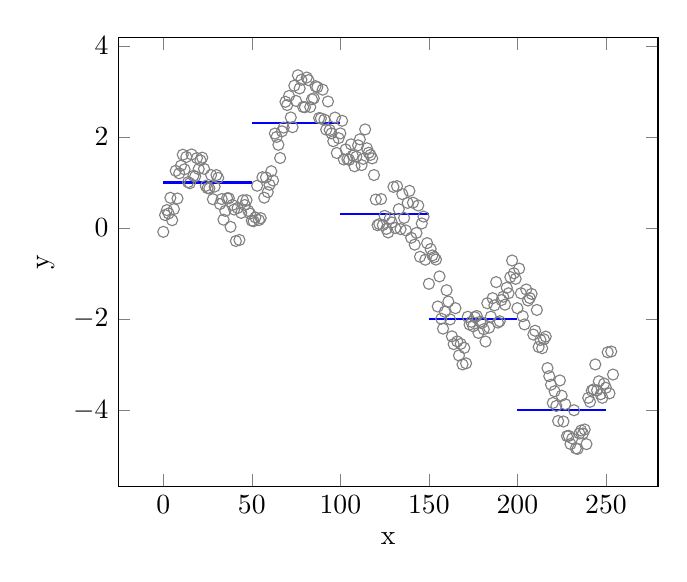
\begin{tikzpicture}
\begin{axis}[%
scatter/classes={%
	a={mark=o,draw=gray}},
xlabel={x},
ylabel={y}
%,
%xticklabels={,,},
%yticklabels={,,}
]
\addplot[scatter,only marks,%
scatter src=explicit symbolic]%
table[meta=label] {
	x y label
0 -0.0835160242859274  a
1 0.285568934387078  a
2 0.394579101186943  a
3 0.319456011084284  a
4 0.663787821139718  a
5 0.172388397197294  a
6 0.415525883567572  a
7 1.2558843677376  a
8 0.648844252387028  a
9 1.20117942302646  a
10 1.37047603500141  a
11 1.60972337793055  a
12 1.28911192846088  a
13 1.56031080227344  a
14 1.00638248369854  a
15 0.984246086186816  a
16 1.61625921176936  a
17 1.14765390737154  a
18 1.13367303859185  a
19 1.53545813877587  a
20 1.29462647613912  a
21 1.48594938329369  a
22 1.54546652597812  a
23 1.30075626330351  a
24 0.924780725901792  a
25 0.876653467885566  a
26 0.868665008436964  a
27 1.16370842893904  a
28 0.632732011300313  a
29 0.910259724400004  a
30 1.16219661138681  a
31 1.1008670138421  a
32 0.526987032463432  a
33 0.636180665523263  a
34 0.183851565842274  a
35 0.375588325804044  a
36 0.653835219246611  a
37 0.653046301882522  a
38 0.025952382432643  a
39 0.506237835066696  a
40 0.406508096522012  a
41 -0.284979202944553  a
42 0.441617462853366  a
43 -0.261760379385229  a
44 0.333222419824161  a
45 0.608838475955039  a
46 0.506281967150246  a
47 0.612056507974025  a
48 0.377464089267289  a
49 0.318273150014862  a
50 0.160728241545451  a
51 0.149920991073773  a
52 0.234019446415594  a
53 0.929124473902112  a
54 0.174356963261225  a
55 0.21750907289469  a
56 1.11559149778506  a
57 0.666788690482064  a
58 1.1108994162566  a
59 0.789282054504515  a
60 0.949495578473449  a
61 1.24609024287059  a
62 1.0439689383038  a
63 2.0738032175923  a
64 2.00021885098137  a
65 1.82646297140817  a
66 1.53750375053874  a
67 2.12319951961666  a
68 2.20452596942365  a
69 2.77103151086561  a
70 2.6996241669188  a
71 2.89934425580715  a
72 2.42736370696646  a
73 2.21425717093992  a
74 3.1240761414546  a
75 2.79047215541272  a
76 3.35357788576053  a
77 3.06462581275212  a
78 3.25621667858734  a
79 2.65606834912304  a
80 2.65170938178788  a
81 3.30359897359816  a
82 3.24693918137054  a
83 2.6567775906426  a
84 2.82500878652476  a
85 2.84711065352786  a
86 3.11358688446847  a
87 3.09279924916506  a
88 2.41591744253837  a
89 2.40630980085128  a
90 3.037289616929  a
91 2.37940869990215  a
92 2.15993843587786  a
93 2.77768389042592  a
94 2.15155270292113  a
95 2.07769601288223  a
96 1.90690445719062  a
97 2.42502603913297  a
98 1.64768546107142  a
99 1.97305051518811  a
100 2.07749159503648  a
101 2.35429938200758  a
102 1.50443150226202  a
103 1.72591064257131  a
104 1.51359098360733  a
105 1.49705886968687  a
106 1.83741092845341  a
107 1.5901074953636  a
108 1.35674404320374  a
109 1.56577833681282  a
110 1.81587205071571  a
111 1.94639450565719  a
112 1.38145985457197  a
113 1.518824266064  a
114 2.16497044046184  a
115 1.75152454886146  a
116 1.65343895  a
117 1.60452768713676  a
118 1.52887  a
119 1.16346422492016  a
120 0.62567950418891  a
121 0.0617660779505969  a
122 0.0874130559773345  a
123 0.636246310715329  a
124 0.065931420837905  a
125 0.266933389091442  a
126 -0.0187439220090775  a
127 -0.0965087727913103  a
128 0.215647966794353  a
129 0.123426863029565  a
130 0.903224120057837  a
131 0.000716092782753586  a
132 0.919853450296996  a
133 0.414521310074015  a
134 -0.0239557141624512  a
135 0.744421694481854  a
136 0.222568307115783  a
137 -0.0516699323132284  a
138 0.552116727206714  a
139 0.816264725585684  a
140 -0.21322574585225  a
141 0.556972587703088  a
142 -0.364064165652314  a
143 -0.106444775224954  a
144 0.494334064171592  a
145 -0.630523341009548  a
146 0.10091122698353  a
147 0.251485628293903  a
148 -0.694754468553538  a
149 -0.330634462175158  a
150 -1.22386964907777  a
151 -0.460814841690383  a
152 -0.600979046426481  a
153 -0.637546556795358  a
154 -0.691924402320308  a
155 -1.72239511476575  a
156 -1.06126261095336  a
157 -1.99039620129457  a
158 -2.20762669760753  a
159 -1.83641583911109  a
160 -1.36503154749765  a
161 -1.61305348642141  a
162 -2.00492559158406  a
163 -2.37670630930511  a
164 -2.54764689092713  a
165 -1.75859506579145  a
166 -2.48808753905506  a
167 -2.79628780843111  a
168 -2.54246577581102  a
169 -2.99359631841596  a
170 -2.63023243383767  a
171 -2.96961812391381  a
172 -1.94707443090953  a
173 -2.1191392756945  a
174 -2.05823633738729  a
175 -2.15585085439569  a
176 -1.95754764171644  a
177 -1.92977651096822  a
178 -2.30121753374042  a
179 -2.05512077363031  a
180 -2.07841025295281  a
181 -2.22054002107119  a
182 -2.49052823895731  a
183 -1.6500262714702  a
184 -2.18659764135757  a
185 -1.9456184006092  a
186 -1.53888803367664  a
187 -1.69660847681546  a
188 -1.18698964913457  a
189 -2.07456341874383  a
190 -2.0453887798746  a
191 -1.58061223276717  a
192 -1.5072742650618  a
193 -1.68141803383867  a
194 -1.31140627053556  a
195 -1.43173297908125  a
196 -1.07619946377905  a
197 -0.712681362673109  a
198 -0.992644450979355  a
199 -1.11508761295528  a
200 -1.75934427392106  a
201 -0.889907055516884  a
202 -1.43146357298287  a
203 -1.93476802335877  a
204 -2.11464198354733  a
205 -1.34866493998177  a
206 -1.59040358835008  a
207 -1.5359533704895  a
208 -1.4454749544856  a
209 -2.33825520330615  a
210 -2.25373298405192  a
211 -1.79731093417145  a
212 -2.61019870508052  a
213 -2.4560855332043  a
214 -2.63723998084539  a
215 -2.44225632768435  a
216 -2.38277372974931  a
217 -3.07383448990287  a
218 -3.25058158518176  a
219 -3.43847567938352  a
220 -3.8396760472169  a
221 -3.58253451343706  a
222 -3.90411063143155  a
223 -4.23479710460466  a
224 -3.34476936812928  a
225 -3.67984879142745  a
226 -4.2454842520664  a
227 -3.86529398324425  a
228 -4.56723044702059  a
229 -4.5617398320318  a
230 -4.74043676227416  a
231 -4.61830041731139  a
232 -3.998853175195  a
233 -4.83718294916592  a
234 -4.84698107957931  a
235 -4.50950485401081  a
236 -4.44364534968019  a
237 -4.5106354052397  a
238 -4.42164548253201  a
239 -4.74294782679374  a
240 -3.72734344634738  a
241 -3.81452325776479  a
242 -3.5682339220494  a
243 -3.54258694402267  a
244 -2.99375368928467  a
245 -3.56406857916209  a
246 -3.36306661090856  a
247 -3.64874392200908  a
248 -3.72650877279131  a
249 -3.41435203320565  a
250 -3.50657313697043  a
251 -2.72677587994216  a
252 -3.62928390721725  a
253 -2.710146549703  a
254 -3.21547868992598  a


};
\addplot[blue, thick] coordinates {(0,1) (50,1)};
\addplot[blue, thick] coordinates {(50,2.3) (100,2.3)};
\addplot[blue, thick] coordinates {(100,0.3) (150,0.3)};
\addplot[blue, thick] coordinates {(150,-2) (200,-2)};
\addplot[blue, thick] coordinates {(200,-4) (250,-4)};
\end{axis}
\end{tikzpicture}

Erweiterung: lineare /quadratische/kubische/.. Funktionen

\underline{Beispiel:}
\[Y_i= \sum\limits_{j=1}^{p}(a_j x_i^3 + b_j x_i^2 + c_j x_i + d_j) \mathbbm{1}_{[\alpha_j,\alpha_{j+1})} (x_i) + \epsilon_i  \; i \in \{1,...,n\} \]
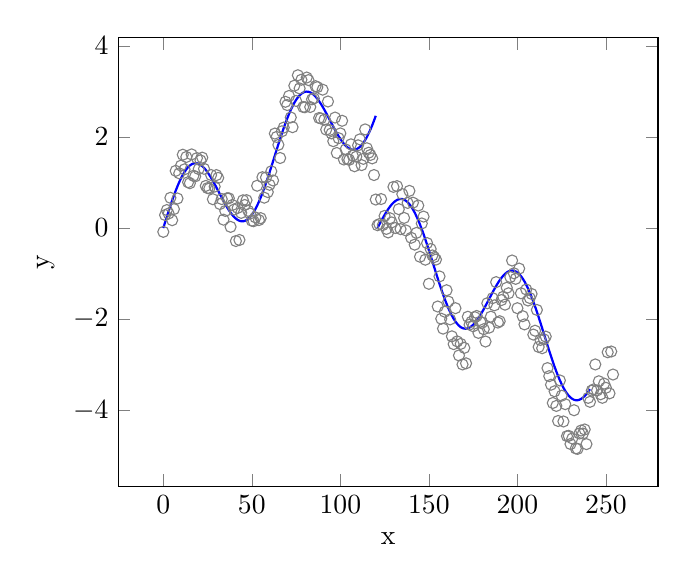
\begin{tikzpicture}
\begin{axis}[%
scatter/classes={%
	a={mark=o,draw=gray}},
xlabel={x},
ylabel={y}
%,
%xticklabels={,,},
%yticklabels={,,}
]
\addplot[scatter,only marks,%
scatter src=explicit symbolic]%
table[meta=label] {
	x y label
0 -0.0835160242859274  a
1 0.285568934387078  a
2 0.394579101186943  a
3 0.319456011084284  a
4 0.663787821139718  a
5 0.172388397197294  a
6 0.415525883567572  a
7 1.2558843677376  a
8 0.648844252387028  a
9 1.20117942302646  a
10 1.37047603500141  a
11 1.60972337793055  a
12 1.28911192846088  a
13 1.56031080227344  a
14 1.00638248369854  a
15 0.984246086186816  a
16 1.61625921176936  a
17 1.14765390737154  a
18 1.13367303859185  a
19 1.53545813877587  a
20 1.29462647613912  a
21 1.48594938329369  a
22 1.54546652597812  a
23 1.30075626330351  a
24 0.924780725901792  a
25 0.876653467885566  a
26 0.868665008436964  a
27 1.16370842893904  a
28 0.632732011300313  a
29 0.910259724400004  a
30 1.16219661138681  a
31 1.1008670138421  a
32 0.526987032463432  a
33 0.636180665523263  a
34 0.183851565842274  a
35 0.375588325804044  a
36 0.653835219246611  a
37 0.653046301882522  a
38 0.025952382432643  a
39 0.506237835066696  a
40 0.406508096522012  a
41 -0.284979202944553  a
42 0.441617462853366  a
43 -0.261760379385229  a
44 0.333222419824161  a
45 0.608838475955039  a
46 0.506281967150246  a
47 0.612056507974025  a
48 0.377464089267289  a
49 0.318273150014862  a
50 0.160728241545451  a
51 0.149920991073773  a
52 0.234019446415594  a
53 0.929124473902112  a
54 0.174356963261225  a
55 0.21750907289469  a
56 1.11559149778506  a
57 0.666788690482064  a
58 1.1108994162566  a
59 0.789282054504515  a
60 0.949495578473449  a
61 1.24609024287059  a
62 1.0439689383038  a
63 2.0738032175923  a
64 2.00021885098137  a
65 1.82646297140817  a
66 1.53750375053874  a
67 2.12319951961666  a
68 2.20452596942365  a
69 2.77103151086561  a
70 2.6996241669188  a
71 2.89934425580715  a
72 2.42736370696646  a
73 2.21425717093992  a
74 3.1240761414546  a
75 2.79047215541272  a
76 3.35357788576053  a
77 3.06462581275212  a
78 3.25621667858734  a
79 2.65606834912304  a
80 2.65170938178788  a
81 3.30359897359816  a
82 3.24693918137054  a
83 2.6567775906426  a
84 2.82500878652476  a
85 2.84711065352786  a
86 3.11358688446847  a
87 3.09279924916506  a
88 2.41591744253837  a
89 2.40630980085128  a
90 3.037289616929  a
91 2.37940869990215  a
92 2.15993843587786  a
93 2.77768389042592  a
94 2.15155270292113  a
95 2.07769601288223  a
96 1.90690445719062  a
97 2.42502603913297  a
98 1.64768546107142  a
99 1.97305051518811  a
100 2.07749159503648  a
101 2.35429938200758  a
102 1.50443150226202  a
103 1.72591064257131  a
104 1.51359098360733  a
105 1.49705886968687  a
106 1.83741092845341  a
107 1.5901074953636  a
108 1.35674404320374  a
109 1.56577833681282  a
110 1.81587205071571  a
111 1.94639450565719  a
112 1.38145985457197  a
113 1.518824266064  a
114 2.16497044046184  a
115 1.75152454886146  a
116 1.65343895  a
117 1.60452768713676  a
118 1.52887  a
119 1.16346422492016  a
120 0.62567950418891  a
121 0.0617660779505969  a
122 0.0874130559773345  a
123 0.636246310715329  a
124 0.065931420837905  a
125 0.266933389091442  a
126 -0.0187439220090775  a
127 -0.0965087727913103  a
128 0.215647966794353  a
129 0.123426863029565  a
130 0.903224120057837  a
131 0.000716092782753586  a
132 0.919853450296996  a
133 0.414521310074015  a
134 -0.0239557141624512  a
135 0.744421694481854  a
136 0.222568307115783  a
137 -0.0516699323132284  a
138 0.552116727206714  a
139 0.816264725585684  a
140 -0.21322574585225  a
141 0.556972587703088  a
142 -0.364064165652314  a
143 -0.106444775224954  a
144 0.494334064171592  a
145 -0.630523341009548  a
146 0.10091122698353  a
147 0.251485628293903  a
148 -0.694754468553538  a
149 -0.330634462175158  a
150 -1.22386964907777  a
151 -0.460814841690383  a
152 -0.600979046426481  a
153 -0.637546556795358  a
154 -0.691924402320308  a
155 -1.72239511476575  a
156 -1.06126261095336  a
157 -1.99039620129457  a
158 -2.20762669760753  a
159 -1.83641583911109  a
160 -1.36503154749765  a
161 -1.61305348642141  a
162 -2.00492559158406  a
163 -2.37670630930511  a
164 -2.54764689092713  a
165 -1.75859506579145  a
166 -2.48808753905506  a
167 -2.79628780843111  a
168 -2.54246577581102  a
169 -2.99359631841596  a
170 -2.63023243383767  a
171 -2.96961812391381  a
172 -1.94707443090953  a
173 -2.1191392756945  a
174 -2.05823633738729  a
175 -2.15585085439569  a
176 -1.95754764171644  a
177 -1.92977651096822  a
178 -2.30121753374042  a
179 -2.05512077363031  a
180 -2.07841025295281  a
181 -2.22054002107119  a
182 -2.49052823895731  a
183 -1.6500262714702  a
184 -2.18659764135757  a
185 -1.9456184006092  a
186 -1.53888803367664  a
187 -1.69660847681546  a
188 -1.18698964913457  a
189 -2.07456341874383  a
190 -2.0453887798746  a
191 -1.58061223276717  a
192 -1.5072742650618  a
193 -1.68141803383867  a
194 -1.31140627053556  a
195 -1.43173297908125  a
196 -1.07619946377905  a
197 -0.712681362673109  a
198 -0.992644450979355  a
199 -1.11508761295528  a
200 -1.75934427392106  a
201 -0.889907055516884  a
202 -1.43146357298287  a
203 -1.93476802335877  a
204 -2.11464198354733  a
205 -1.34866493998177  a
206 -1.59040358835008  a
207 -1.5359533704895  a
208 -1.4454749544856  a
209 -2.33825520330615  a
210 -2.25373298405192  a
211 -1.79731093417145  a
212 -2.61019870508052  a
213 -2.4560855332043  a
214 -2.63723998084539  a
215 -2.44225632768435  a
216 -2.38277372974931  a
217 -3.07383448990287  a
218 -3.25058158518176  a
219 -3.43847567938352  a
220 -3.8396760472169  a
221 -3.58253451343706  a
222 -3.90411063143155  a
223 -4.23479710460466  a
224 -3.34476936812928  a
225 -3.67984879142745  a
226 -4.2454842520664  a
227 -3.86529398324425  a
228 -4.56723044702059  a
229 -4.5617398320318  a
230 -4.74043676227416  a
231 -4.61830041731139  a
232 -3.998853175195  a
233 -4.83718294916592  a
234 -4.84698107957931  a
235 -4.50950485401081  a
236 -4.44364534968019  a
237 -4.5106354052397  a
238 -4.42164548253201  a
239 -4.74294782679374  a
240 -3.72734344634738  a
241 -3.81452325776479  a
242 -3.5682339220494  a
243 -3.54258694402267  a
244 -2.99375368928467  a
245 -3.56406857916209  a
246 -3.36306661090856  a
247 -3.64874392200908  a
248 -3.72650877279131  a
249 -3.41435203320565  a
250 -3.50657313697043  a
251 -2.72677587994216  a
252 -3.62928390721725  a
253 -2.710146549703  a
254 -3.21547868992598  a


};
\addplot[blue, thick] coordinates {
( 0 , 0 )
( 1 , 0.124833416646828 )
( 2 , 0.248669330795061 )
( 3 , 0.37052020666134 )
( 4 , 0.489418342308651 )
( 5 , 0.604425538604203 )
( 6 , 0.714642473395036 )
( 7 , 0.819217687237691 )
( 8 , 0.917356090899523 )
( 9 , 1.00832690962748 )
( 10 , 1.0914709848079 )
( 11 , 1.16620736006144 )
( 12 , 1.23203908596723 )
( 13 , 1.28855818541719 )
( 14 , 1.33544972998846 )
( 15 , 1.37249498660405 )
( 16 , 1.39957360304151 )
( 17 , 1.41666481045247 )
( 18 , 1.4238476308782 )
( 19 , 1.42130008768741 )
( 20 , 1.40929742682568 )
( 21 , 1.38820936664887 )
( 22 , 1.35849640381959 )
( 23 , 1.32070521217672 )
( 24 , 1.27546318055115 )
( 25 , 1.22347214410396 )
( 26 , 1.16550137182146 )
( 27 , 1.10237988023383 )
( 28 , 1.0349881501559 )
( 29 , 0.964249329213982 )
( 30 , 0.891120008059867 )
( 31 , 0.816580662433291 )
( 32 , 0.74162585657242 )
( 33 , 0.667254305856751 )
( 34 , 0.594458897973168 )
( 35 , 0.52421677231038 )
( 36 , 0.457479556705148 )
( 37 , 0.395163859091507 )
( 38 , 0.338142109057281 )
( 39 , 0.287233840816026 )
( 40 , 0.243197504692072 )
( 41 , 0.206722888935589 )
( 42 , 0.178424227586412 )
( 43 , 0.158834063250545 )
( 44 , 0.148397926110484 )
( 45 , 0.147469882334903 )
( 46 , 0.156308996366536 )
( 47 , 0.175076742435899 )
( 48 , 0.20383539116416 )
( 49 , 0.242547387375668 )
( 50 , 0.291075725336862 )
( 51 , 0.349185317672268 )
( 52 , 0.416545344279847 )
( 53 , 0.492732557776099 )
( 54 , 0.577235512444013 )
( 55 , 0.669459674429608 )
( 56 , 0.768733362127679 )
( 57 , 0.874314457402362 )
( 58 , 0.985397820586244 )
( 59 , 1.10112333516976 )
( 60 , 1.22058450180107 )
( 61 , 1.34283749572791 )
( 62 , 1.4669105971825 )
( 63 , 1.59181390048435 )
( 64 , 1.71654920485049 )
( 65 , 1.84011998808782 )
( 66 , 1.96154136351338 )
( 67 , 2.0798499206166 )
( 68 , 2.19411335113861 )
( 69 , 2.3034397643882 )
( 70 , 2.40698659871879 )
( 71 , 2.50396904012588 )
( 72 , 2.59366786384915 )
( 73 , 2.67543662062856 )
( 74 , 2.74870809581163 )
( 75 , 2.81299997677474 )
( 76 , 2.86791967203149 )
( 77 , 2.913168233877 )
( 78 , 2.94854334537461 )
( 79 , 2.97394134183977 )
( 80 , 2.98935824662338 )
( 81 , 2.99488981084509 )
( 82 , 2.99073055667977 )
( 83 , 2.97717183375629 )
( 84 , 2.95459890808828 )
( 85 , 2.92348711262349 )
( 86 , 2.88439709787411 )
( 87 , 2.83796923008218 )
( 88 , 2.78491719289176 )
( 89 , 2.72602085645788 )
( 90 , 2.66211848524176 )
( 91 , 2.59409836234935 )
( 92 , 2.52288991410025 )
( 93 , 2.44945442350706 )
( 94 , 2.37477542545336 )
( 95 , 2.29984887953819 )
( 96 , 2.22567321877702 )
( 97 , 2.15323937358906 )
( 98 , 2.08352087074807 )
( 99 , 2.01746410622468 )
( 100 , 1.95597888911063 )
( 101 , 1.89992935110712 )
( 102 , 1.85012531240646 )
( 103 , 1.80731419023642 )
( 104 , 1.77217353091435 )
( 105 , 1.74530424002833 )
( 106 , 1.72722457838719 )
( 107 , 1.71836498372981 )
( 108 , 1.71906376993351 )
( 109 , 1.72956374669362 )
( 110 , 1.7500097934493 )
( 111 , 1.78044741179601 )
( 112 , 1.82082227084868 )
( 113 , 1.87098075009791 )
( 114 , 1.93067147433532 )
( 115 , 1.99954782531157 )
( 116 , 2.07717140503129 )
( 117 , 2.16301641608097 )
( 118 , 2.25647491522288 )
( 119 , 2.35686288776297 )
( 120 , 2.46342708199957 )

( 121 , 0 )
( 122 , 0.0748334166468282 )
( 123 , 0.148669330795061 )
( 124 , 0.22052020666134 )
( 125 , 0.28941834230865 )
( 126 , 0.354425538604203 )
( 127 , 0.414642473395035 )
( 128 , 0.469217687237691 )
( 129 , 0.517356090899523 )
( 130 , 0.558326909627483 )
( 131 , 0.591470984807897 )
( 132 , 0.616207360061435 )
( 133 , 0.632039085967226 )
( 134 , 0.638558185417193 )
( 135 , 0.63544972998846 )
( 136 , 0.622494986604054 )
( 137 , 0.599573603041505 )
( 138 , 0.566664810452469 )
( 139 , 0.523847630878195 )
( 140 , 0.471300087687414 )
( 141 , 0.409297426825682 )
( 142 , 0.338209366648874 )
( 143 , 0.25849640381959 )
( 144 , 0.17070521217672 )
( 145 , 0.0754631805511505 )
( 146 , -0.0265278558960435 )
( 147 , -0.134498628178536 )
( 148 , -0.24762011976617 )
( 149 , -0.365011849844095 )
( 150 , -0.485750670786018 )
( 151 , -0.608879991940133 )
( 152 , -0.73341933756671 )
( 153 , -0.85837414342758 )
( 154 , -0.982745694143249 )
( 155 , -1.10554110202683 )
( 156 , -1.22578322768962 )
( 157 , -1.34252044329485 )
( 158 , -1.45483614090849 )
( 159 , -1.56185789094272 )
( 160 , -1.66276615918397 )
( 161 , -1.75680249530793 )
( 162 , -1.84327711106441 )
( 163 , -1.92157577241359 )
( 164 , -1.99116593674945 )
( 165 , -2.05160207388952 )
( 166 , -2.1025301176651 )
( 167 , -2.14369100363346 )
( 168 , -2.1749232575641 )
( 169 , -2.19616460883584 )
( 170 , -2.20745261262433 )
( 171 , -2.20892427466314 )
( 172 , -2.20081468232773 )
( 173 , -2.18345465572015 )
( 174 , -2.1572674422239 )
( 175 , -2.12276448755599 )
( 176 , -2.08054032557039 )
( 177 , -2.03126663787232 )
( 178 , -1.97568554259764 )
( 179 , -1.91460217941376 )
( 180 , -1.84887666483024 )
( 181 , -1.77941549819893 )
( 182 , -1.7071625042721 )
( 183 , -1.6330894028175 )
( 184 , -1.55818609951565 )
( 185 , -1.48345079514951 )
( 186 , -1.40988001191218 )
( 187 , -1.33845863648662 )
( 188 , -1.2701500793834 )
( 189 , -1.20588664886139 )
( 190 , -1.1465602356118 )
( 191 , -1.09301340128121 )
( 192 , -1.04603095987412 )
( 193 , -1.00633213615085 )
( 194 , -0.974563379371435 )
( 195 , -0.951291904188373 )
( 196 , -0.937000023225261 )
( 197 , -0.932080327968514 )
( 198 , -0.936831766123 )
( 199 , -0.951456654625395 )
( 200 , -0.976058658160228 )
( 201 , -1.01064175337662 )
( 202 , -1.05511018915491 )
( 203 , -1.10926944332023 )
( 204 , -1.17282816624371 )
( 205 , -1.24540109191172 )
( 206 , -1.32651288737651 )
( 207 , -1.41560290212589 )
( 208 , -1.51203076991782 )
( 209 , -1.61508280710824 )
( 210 , -1.72397914354212 )
( 211 , -1.83788151475824 )
( 212 , -1.95590163765065 )
( 213 , -2.07711008589975 )
( 214 , -2.20054557649294 )
( 215 , -2.32522457454664 )
( 216 , -2.45015112046181 )
( 217 , -2.57432678122298 )
( 218 , -2.69676062641094 )
( 219 , -2.81647912925193 )
( 220 , -2.93253589377532 )
( 221 , -3.04402111088937 )
( 222 , -3.15007064889288 )
( 223 , -3.24987468759354 )
( 224 , -3.34268580976358 )
( 225 , -3.42782646908565 )
( 226 , -3.50469575997167 )
( 227 , -3.57277542161281 )
( 228 , -3.63163501627019 )
( 229 , -3.68093623006649 )
( 230 , -3.72043625330638 )
( 231 , -3.7499902065507 )
( 232 , -3.76955258820399 )
( 233 , -3.77917772915132 )
( 234 , -3.77901924990209 )
( 235 , -3.76932852566468 )
( 236 , -3.75045217468843 )
( 237 , -3.72282859496871 )
( 238 , -3.68698358391903 )
( 239 , -3.64352508477712 )
( 240 , -3.59313711223703 )
( 241 , -3.53657291800043 )
};
\end{axis}
\end{tikzpicture}

\underline{Problem:} 
\begin{itemize}
 \item Unstetigkeiten an Intervallgrenzen
 \item (asymptotische) Verhalten an den Intervallgrenzen kann (insbesondere bei Polynomen höherer Ordnung) sehr unpassend sein
\end{itemize}

%Vorlesung vom 21.11.17

	\textbf{Wünsche: } \begin{itemize}
		\item stetige Übergänge an den Intervallgrenzen
		\item keine Knicke an den Intervallgrenzen
		\item [$\rightarrow$] glatter Übergang
	\end{itemize}

\subsection{Splines (polynome der Ordnung M)}
''Spline'' $\approxeq$ Polynomzug
\todo{Glätten Sprünge der Regressionsfunktionen s.o.}

\begin{itemize}
	\item $ \alpha_1 < \ldots < \alpha_r $
	\item[$\rightarrow$] $(r+1) \text{ Intervalle }  (-\infty, \alpha_1),[\alpha_1, \alpha_2) , \ldots, [\alpha_{r-1} , \alpha_r), [\alpha_r, \infty)$
	\item $Y_i  = \sum_{j=1}^{r} \theta_j h_j (x_i) + \epsilon_i$ , $i \in {1,\ldots,n}$
	\item [] 
	\begin{itemize}
		\item mit $h_1(x):=x^0$
		\item $h_2(x) := x^1$
		\item $h_{M+1}(x) := x^{M}$
		\item $h_{M+2}(x) := (x- \alpha_1)^{M}_{+}$
		\item $h_{M+r+1}(x) := (x- \alpha_r)^{M}_{+}$
	\end{itemize} 

\item[$\rightarrow$] Ableitungen bis zur Ordnung (M-1) in den Knoten stetig
\end{itemize}
\underline{Üblich:} 
\begin{itemize}
	\item Knoten wählt man äquidistant oder gemäß der Quantile
	\item $M \in \{0,1,3\}$
\end{itemize}

\chapter{Modellwahl und Regularisierung}
\underline{Hier:} Multiple lineare Regression 
\[ Y_{i} = \beta_{0} + \beta_{1} x_{i}^{(1)} + ... \beta_{k} x_{i}^{(k)} + \epsilon_{i} i \in \{ 1,...,n \} \]
Schätzer für $\beta_{j}$ über kleinste-Quadrate-Methode\\
\underline{Problem:}
\begin{itemize}
 \item $n \approx k$
 \item $k > n$
\end{itemize}
$\rightarrow$ 
\begin{itemize}
 \item $k > n$: keine eindeutige Lösung
 \item hohe Varianz bei den Schätzern $\widehat{\beta_j}$
 \item schlechte Qualität bei Vorhersagen
\end{itemize}

\underline{Lösung:}
\begin{itemize}
 \item eliminieren irrelevanter Variablen
 \item zusätzliche Bedingungen in das Modell einfügen
\end{itemize}

\section{Modellwahl}
\subsection{Modellbewertung}
\paragraph{Residual Sum of Squares(RSS)}
\[ \text{RSS}:= \sum\limits_{i=1}^{n} (y_i \hat{y_i})^2 \text{ mit} \]
\[ \hat{y}_i =  \hat{\beta_{0}} + \hat{\beta_{1}} x_{i}^{(1)} + ... \hat{\beta_{k}} x_{i}^{(k)} + \epsilon_{i} i \in \{ 1,...,n \} \]
$\rightarrow$ ``je kleiner desto besser''

%Vorlesung vom 30.11.17
\paragraph{Mallow's Cp}
\[ \text{Cp}= \frac{1}{n}(\text{RSS} + 2k \hat{\sigma}^{2} \]
mit $\hat{\sigma}^{2}$ als Varianzschätzer für $\epsilon_i , i \in \{1,\dots,n\}$ \\
(Voraussetzung ``Homoskedastizität'')\\
$\Rightarrow$ ``Je kleiner desto besser''
\paragraph{Akarkas Informationskriterium (AIC) }
\[ \text{AIC} := n \log (\hat{b}^2) + 2k \]
$\Rightarrow$ ``Je kleiner desto besser''

\paragraph{Bayes'sche Informationskriterium (BIC)}
\[ \text{BIC} := n \log (\hat{b}^2) + k \cdot \log(n) \]
$\Rightarrow$ ``Je kleiner desto besser''

\paragraph{Bestimmtheitsmaß ($R^2$)}
\[ R^2 := 1 - \frac{RSS}{TSS} \]
mit 
\[ TSS := \sum\limits_{i=1}^n (y_i - \bar{y_n} )^2 \]
mit
\[ \bar{y}_n = \frac{1}{n} \sum\limits_{i=1}^{n}y_i \]
$\Rightarrow$ ``Je größer desto besser'' \\
\underline{Bemerkung:} Man kann zeigen:
\[ 0 \leq \text{RSS} \leq \text{TSS} \]

\paragraph{Korrigiertes Bestimmtheitsmaß ($R^{2}_{adj}$)}
\[ R_{adj}^{2} := 1 - \frac{\frac{\text{RSS}}{n-k-1}}{\frac{\text{TSS}}{n-1}} \]
$\Rightarrow$ ``Je größer desto besser'' \\
\underline{Bemerkung:} RSS und $R^{2}$ hängen stark von der Anzahl der Einflussgrößen (k) ab\\
$\Rightarrow$ RSS und $R^{2}$ nur zum Vergleich von Modellen mit gleicher Anzahl von Einflussgrößen geeignet

\section{Modellwahlverfahren}
\subsection{Best Subset Selection}
vergleiche alle möglichen (Sub-)Modelle miteinander
\[ \{ x^{(j_1)},\dots, x^{(j_l)}\} \subseteq \{x^{(1)}, \dots, x^{k} \} \]
mit 
$l \in \{1, \dots, k \} $
\[ \Rightarrow Y_i = \beta_0 + \beta_1 x_i^{(j_1)} + \dots + \beta_l x_i^{(j_l)} + \epsilon_i , i \in \{1,..n\} \]
$\Rightarrow 2^{k} $ Möglichkeiten der Modellbildung
\underline{Vorgehen}
\begin{enumerate}
	\item Berechne Null-Modell $\mathcal{M}_0 $:
		$Y_i= \beta_0 + \epsilon_i , i \in \{1,\dots,n\} $
	\item Für $l=1,\dots,k$:
		\begin{enumerate}
			\item Berechne alle $\binom{k}{l}$ Modell mit (genau) $l$ Einflussgrößen
			\item Wähle unter allen diesen Modellen das mit dem größten $R^{2} (\mathcal{M}_0)$
		\end{enumerate}
	\item Wähle unter $\mathcal{M}_0,\dots,\mathcal{M}_k$ das beste Modell gemäß
		\begin{itemize}
			\item kreuzvalidierter Vorhersagefehle (später)
			\item AIC
			\item BIC
			\item $R^2$
		\end{itemize}
\end{enumerate}
\underline{ABER:} Falls $k$ zu groß ist, wird Best Subset Selection zu teuer \\
Beispiel: $k=20 \Rightarrow 1.048.576$ Modelle müssen berechnet werden

\subsection{Vorwärtsselektion}
\underline{Vorgehen:} 
\begin{enumerate}
	\item Berechne das Null-Modell $\mathcal{M}_0$
	\item Für $l=0,\dots,(k-1)$
		\begin{enumerate}
			\item Berechne alle $(k-l)$ Modelle, welche das Modell $\mathcal{M}_i$ mit einem zusätzlichen Parameter bzw. Einflussgrößen betrachten
			\item Wähle unter allen diesen Modellen das mit dem größten $R^{2} (\mathcal{M}_{l+1})$
		\end{enumerate}
	\item Wähle unter $\mathcal{M}_0,\dots,\mathcal{M}_k$ das beste Modell gemäß:
		\begin{itemize}
			\item kreuzvalidierter Vorhersagefehler
			\item AIC
			\item BIC
			\item \dots
		\end{itemize}
\end{enumerate}
\underline{Vorteil:} weniger rechenintensiv:
\[ 1 + \sum\limits_{l=0}^{k-1} (k-l)=1+ \frac{k(k+1)}{2} \text{ Modelle}\]
Beispiel: $k=20 \Rightarrow 211$ Modelle müssen berechnet werden \\ \\
\underline{Nachteil:} Vorwärtsselektion ``übersieht'' viele Modelle  \\
\underline{Beachte:} Falls $k > n$, ist der Algorithmus bei $l=n-1$ abzubrechen, da sonst keine eindeutigen Lösungen mehr entstehen

\subsection{Rückwärtsselektion}
\underline{Vorgehen:}
\begin{enumerate}
	\item Berechne das ``volle'' Modelle $(\mathcal{M}_k)$
	\item Für $l=k,\dots,1:$
		\begin{enumerate}
			\item Berechne alle $l$ Modelle, welche alle Einflussgrößen aus $\mathcal{M}_l$ außer einem enthalten
			\item Wähle unter allen diesen Modellen das mit dem größten $R^{2} (\mathcal{M}_{l+1})$
		\end{enumerate}
	\item Wähle unter $\mathcal{M}_0,\dots,\mathcal{M}_k$ das beste Modell gemäß:
		\begin{itemize}
			\item kreuzvalidierter Vorhersagefehler
			\item AIC
			\item BIC
			\item \dots
		\end{itemize}
\end{enumerate}
\underline{Beachte:} Hier muss $k < n$ gelten!

\section{Regularisierung (Shrinkage)}
\subsection{Ridge-Regression}
\[ \lambda > 0 \]
\[ \sum\limits_{i=1}^{n} (y_i - \beta_0 - \beta_1 x_i^{(1)} - \dots - \beta_i x_i^{(k)})^2 + \underbrace{\lambda \sum\limits_{j=1}^{k} \beta_j^{2}}_{``Strafterm''} \rightarrow min \]
	Zusatzterm sorgt dafür, dass (betragsmäßig) große $\beta_i$ vermieden werden \\
	$\lambda$ heißt \underline{Tuning-Parameter} und steuert die Stärke der Bestrafung für betragsmäßig große $\beta_0 \beta_j$
	\begin{itemize}
		\item $\lambda=0$ übliche Regression mit KQM
		\item $\lambda >>0$: Bestrafung betragsmäßig großer $\beta_j$ bekommt ``Übergewicht'', das heißt $||\hat{\beta}||_2 \rightarrow 0 $ für $\lambda \rightarrow \infty $
			\[ ||\beta ||_2 := \sqrt{\sum\limits_{j=1}^{k}\beta_j^{2}} \]
	\end{itemize}
	\underline{Beobachtung:}
	\begin{itemize}
		\item bei linearer Regression hängt der Wert $\hat{\beta}_j x^{(j)}$ nicht von der Skalierung der Einflussgröße $x^{(j)}$ ab
		\item bei Ridge-Regression gilt das nicht mehr!
	\end{itemize}
$\Rightarrow$ Ausweg: Standardisierung vor der Modellberechnung gemäß:
\[ \tilde{X}_i^{(j)} := \frac{x_i^{(j)}}{\sqrt{\frac{1}{n}\sum\limits_{i=1}^{n}(x_i^{(j)} - \bar{x}^{(j)}_n})} \]
$\Rightarrow $ alle $\tilde{x}^{(j)}$ haben Varianz 1 und sind unabhängig der Skalierung der $x^{(j)}$ \\
$\Rightarrow$ ``Schrumpfen'' der Parameter $\hat{\beta_j}$ aber nicht ``0'' \\
$\Rightarrow$ Reduktion der Varianz der Schätzer (``Glättung'')

\subsection{Lasso (Least Absolute Shrinkage and Selection Operator)}
Ähnlich wie Ridge Regression 
\begin{itemize}
	\item \(\lambda > 0 \)
	\item \(\sum_{i = 1}^{n}(y_i -\beta_0 - \beta_1 x_i^{(1)} - \ldots - \beta_k x_i^{(k)})^2 + \underbrace{\lambda \sum_{j = 1}^{k}|\beta_j|}_{Strafterm}
	\rightarrow_{\beta_0, \ldots, \beta_k \in \mathbb{R}} \min \)
	\item Bestrafungsterm in L$^1$-Norm (Ridge Regression L$^2$ Norm)
	\item Hauptunterschied zur Ridge Regression: $L^1$-Norm führt dazu, dass viele Koeffizienten "`=0"' geschätzt werden (Ridge-Regression "'$\approx$ 0"')
	\item einfachere Interpretierbarkeit des Modells
	\item [\(\rightarrow\)] Variablenselektion
	\item [ABER]
	\begin{itemize}
		\item Varianz der $ \hat{\beta_j} $ ist bei Lasso größer als bei Ridge
	\end{itemize}
\end{itemize}

%L^1 Norm von \beta := (\beta_1, \ldots,\beta_i)
%Allgemein: L$^P$-Norm von $\beta$\\
%\(\rightarrow ||\beta||_p = ||\beta||_{L^p} = \sqrt{\sum_{j = 1}^{k} |\beta_j|^p}\)\\
%\(\Leftrightarrow ||\beta||_p^p = \sum_{j=1}^{k}|\beta_j|^P\)

\subsection{Wahl des Tuningparameters $\lambda$}
\textbf{Kreuzvalidierung:}
\begin{enumerate}
	\item Wähle ein Gitter von möglichen $\lambda$-Werten
	\item Berechne für jeden dieser Werte den Kreuzvalidierten Fehler
	\item Wähle das \(\lambda\) mit dem kleinsten Fehler
	\item Berechne mit dem "`finalen"' \( \lambda \) das Modell erneut (mit kompletten Datensatz)
\end{enumerate}


\section{Kreuzvalidierung}
\textbf{\underline{Beispiel:}}
	\begin{itemize}
		\item ($X_i$, $Y_i$)$_{i=1}^n$ - Stichprobe
		\item $X_i$ Körpergröße
		\item $Y_i$ -Körpergewiche
		\item Modell: 
	\end{itemize}
		\[Y_I = \beta_0 + \beta_1 x_i\epsilon_i \text{ ; } i \in \{1, \ldots,n\}\]
\begin{itemize}
\item bestimmen $\hat{\beta_0}$ und $\hat{\beta_1}$ über KQM
\item [\(\rightarrow\)] Wie gut sind die Schätzungen
\end{itemize}


\[ MSE := \frac{1}{n} \sum_{i = 1}^{n} (y_i - \hat{y_i})^2 \text{  (Mean Squared Error)}\]

\begin{itemize}
	\item[\( \rightarrow \)] gilt nur für vorliegende Stichprobe
	\item[\( \rightarrow \)] Wie gut sind diese Schätzungen für zukünftige Daten?
\end{itemize}

\subsection{Vorgehen}
\begin{itemize}
	\item Man verwendet einen Teil der Stichprobe als \underline{Trainingssatz} und den anderen Teil als \underline{Validierungsdatensatz}
	\item[\( \rightarrow \)] Den Trainingsdatensatz zum Schätzen der Parameter
	\item[\( \rightarrow \)] Den Validierungsdatensatz zum Überprüfen der Vorhersagegüte
\end{itemize}

\textbf{\underline{Beispiel}(Fortsetzung):}
\begin{itemize}
	\item $(x_i, y_i)_i \in I_T$ - Trainingsdaten
	\item $(x_i,y_i)_i \in I_V$ -Validierungsdaten
\end{itemize}
mit $ I_T $, $ I_V $   $\{1,\ldots,n\}$   und $I_T \cap I_V = \emptyset$
	
\begin{itemize}
	\item $ \hat{\beta_0}^T $, $ \hat{\beta_1}^T $ - Schätzer für $\beta_0$ und  $\beta_1$ unter Verwendung von $ (x_i $, $ Y_i $$ )_{i \in I_T} $
	\item mittlerer quadratischer Fehler über Validierungsdaten
\end{itemize}

\[MSE_V := \frac{1}{|I_V|} \sum_{i \in I_V}(Y_i - \underbrace{(  \hat{\beta_0}^T +  \hat{\beta_1}^T x_i)}_{:= \hat{y_i}^{(T)}})^2\]

\textbf{Problem:} Bias durch "`ungünstige"' Aufteilung in Trainings und Validierungsdaten $\rightarrow$
unter bzw. Überschätzen des MSE

\textbf{Lösung:} m-maliges Aufteilen der gesamten Stichprobe in Trainings und Validierungsdaten

für \(L=1,\ldots, m\) jeweils Parameter schätzen und mittleren quadratischen Fehler berechnen. Anschließend mittleren quadratischen Fehler (MSE) bestimmen

$\rightarrow$ Aufteilung jeweils möglichst zufällig wählen

\textbf{\underline{Beispiel}(Fortsetzung):}
\begin{itemize}
	\item m mal in trainings und Validierungsdaten aufteilen
	\item $ (x_i, y_i)_{i \in I_T^{(1)}} , (x_i,y_i)_{i \in I_V^{(1)}} $ $ \ldots $
	\item $ (x_i, y_i)_{i \in I_T^{(m)} }, (x_i,y_i)_{i \in I_V^{(m)}} $
	\item bestimmen jeweils  $\hat{\beta_0}^{T,L}$, $\hat{\beta_1}^{T,L}$ und 
	\[ MSE_V^{(l)} := \frac{1}{|I_V^{(l)}|} \sum_{i \in I_V^{(1)}}(y_i - (\hat{\beta_0}^{(T,l)} + \hat{\beta_1}^{(T,l)} x_i))^2  \]
	\item für $l = 1, \ldots, m$
	\item bestimme den gemittelten MSE
	\[MSE_V^m := \frac{1}{m} \sum_{1}^{m} MSE_V^{(l)}\]
\end{itemize}

\subsection{Mögliche Aufteilungen}
\subsubsection{Leave one out Cross Validation}
\textbf{\underline{Beispiel}(Fortsetzung):}
\begin{itemize}
	\item für \(l = 1,\ldots,n\) 
	\item $(x_i, y_i)_i \in \{1, \ldots, n \} \setminus \{l\}$ Trainingsdatensatz
	\item $(x_i, y_i)_i = l$ Validierungsdatensatz
	\[MSE_V^{(l)} = (y_l - (\hat{\beta_0}^{(T, \{l\})} + \hat{\beta_1}^{(T, \{l\})} x_i)) \text{ für } l = 1,\ldots ,n\]	
	\[MSE_v^n := \frac{1}{n}\sum_{l = 1}^{n} MSE_V^{(l)}\]
\end{itemize}

\subsubsection{k-fache Kreusvalidierung}
\textbf{\underline{Beispiel} (Fortsetzung):}

Aufteilung in K Blöcke:
\[(x_i, y_i)_{i \in I^{(k)}} \text{ für }  k = 1, .., K \] 
\[\text{mit } I^{(k_1)} \cup I^{(k_2)} = \emptyset \text{ für } k_1, k_2 \in {1, \ldots ,K} \text{ mit } k_1 \neq k_2 \]
\[ \text{und } |I^{(K)}| = \begin{cases}
\frac{n}{m} &, n \mod K= 0\\
n \mod K &, n \mod K \neq 0
\end{cases}
\]
\[\text{und } |I^{(k)}| = \frac{n - |I^{(k)}|}{K-1} \text{ für } k = \{1, \ldots ,K\} \]

möglichst \(|I^{(K)}| \approx |I^{(k)}|\)für \(k = \{1, \ldots ,K-1\}\)\\


Für \(k = 1, \ldots, K\) 
\begin{itemize}
	\item[] \((x_i, y_i)_{ i \in I^{(l)}}, l \in \{1, \ldots, K\}\setminus \{k\}\) - Trainingsdaten
	\item[] \((x_i, y_i)_{ i \in I^{(k)}} \) - Validierungsdatensatz
	\item Bemerkung \(K=n \rightarrow LOOCV\) 	
	\item[\(\rightarrow\)]\(MSE_V^{(k)} = \frac{1}{|I^{(k)}|} \sum_{i \in I^{(k)}} ( y_i -( \hat{\beta_0}^{(T,k)} + \hat{\beta_1}^{(T,k)}  x_i))^2\) 
	\item [\(\rightarrow\)]
	\(MSE_V^K = \frac{1}{K} \sum_{k=1}^{K} MSE_V^{(k)}\) 
	\item üblich K=5 oder K=10
\end{itemize}

\section{Kurzzusammenfassung}
Multiple Lineare Regression
\[Y_I = \beta_0 + \beta_1 x_i^{(1)} + \ldots + \beta_k x_i^{(k)} + \epsilon_i \text{ ; } i \in \{1, \ldots,n\}\]

\textbf{Problemfälle}
\begin{itemize}
	\item \(n \approx k\)
	\item \(n < k\)
\end{itemize}
\textbf{Auswege:} \\
Variablenselektion
\begin{itemize}
	\item[\(\rightarrow\)] BSS
	\item[\(\rightarrow\)] VS (Vorwärtsselektion)
	\item[\(\rightarrow\)] RS (Rückwärtsselektion)
\end{itemize}
Regularisierung
\begin{itemize}
	\item RR (Tuning Parameter (\(\lambda > 0\) für die Stärke der Bestrafung)
	\item Lasso
\end{itemize}
\todo{\(AIC = AC + f(k^2)\)}
\todo{\(Cp: K:= {0, \ldots, k}\)\\
\(P<= K\) \\
\(|P| = p C_p\) \(\approx p \rightarrow\) dieses Modell "`am besten"' geeignet}

Modellbewertung:RSS, Mallows Cp, AIC, BIC, $R^2$ $R_adj^2$



\chapter{Grundlagen der Versuchsplanung}
Alle gewonnenen Beobachtungen für Y unterliegen einer Vielzahl von unterschiedlichen Einflußfaktoren. Einige davon sind bekannt (und können quantifiziert werden), andere dagegen sind unbekannt oder wirken zufällig auf die Beobachtungen $y_1,\cdots,y_n$ \\
		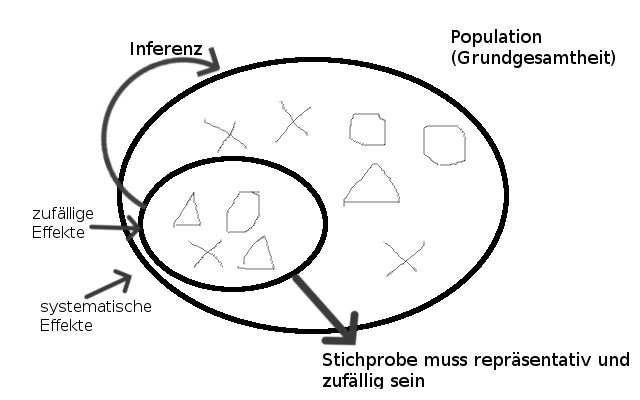
\includegraphics[scale=0.5]{VorlesungenTexDateien/images/Stichprobe}

$\Rightarrow$ alle systematischen Effekte sollten bei der Versuchsplanung mit berücksichtigt werden 
Es müssen 3 Bedingungen erfüllt sein:
\begin{enumerate}
	\item Randomisierung von Proben/Individuen zwischen den Kategorien einer kategorialen Variable
	\item Es muß auf eine ausreichende Anzahl von Replikaten geachtet werden
	\item Falls systematische Effekte bei der Versuchsdurchführung auftreten können, müssen diese bei der Verteilung der Proben auf die Prozessierungsblöcke berücksichtgt werden (\underline{Blocking})
\end{enumerate}


\end{document}
